%===============================================================================
% ifacconf.tex 2022-02-11 jpuente  
% 2022-11-11 jpuente change length of abstract
% Template for IFAC meeting papers
% Copyright (c) 2022 International Federation of Automatic Control
%===============================================================================
\documentclass{ifacconf}

\usepackage{hyperref}
\usepackage{graphicx}      % include this line if your document contains figures
\graphicspath{ {./images/} }
\usepackage{caption}
\usepackage[square,sort&compress,sectionbib,numbers]{natbib}        % required for bibliography
\usepackage{glossaries}    % required for glossary
\usepackage{cuted}
\usepackage{float}
\usepackage{listings}
\usepackage{xcolor}
\usepackage{pgfgantt}
\usepackage{multirow}
\usepackage{array} 
\makeglossaries
\loadglsentries{glossary}  % loading the glossary.tex file

\definecolor{codegreen}{rgb}{0,0.6,0}
\definecolor{codegray}{rgb}{0.5,0.5,0.5}
\definecolor{codepurple}{rgb}{0.58,0,0.82}
\definecolor{backcolour}{rgb}{0.95,0.95,0.92}

\lstdefinestyle{mystyle}{
	backgroundcolor=\color{backcolour},   
	commentstyle=\color{codegreen},
	keywordstyle=\color{magenta},
	numberstyle=\tiny\color{codegray},
	stringstyle=\color{codepurple},
	basicstyle=\ttfamily\footnotesize,
	breakatwhitespace=false,         
	breaklines=true,                 
	captionpos=b,                    
	keepspaces=true,                 
	numbers=left,                    
	numbersep=5pt,                  
	showspaces=false,                
	showstringspaces=false,
	showtabs=false,                  
	tabsize=2
}

\lstset{style=mystyle}

%===============================================================================
\begin{document}
	
	\begin{frontmatter}
		
		\title{Methods of Reducing Computational Requirements for Large Language Models} 
		% Title, preferably not more than 10 words.
		
		\author[First]{Oleksandr Kononov} 
		
		\address[First]{South East Technological University, 
			Cork Road, Waterford, Ireland (e-mail: 20071032@mail.wit.ie).}
		\begin{abstract}                % Abstract of 50--100 words
			The increasing computational requirements of \glspl{llm} poses significant challenges to their deployment and accessibility, especially for consumers and small organisations with limited compute resources. This research aims to investigate viable and efficient \gls{llm} compression methods such as \gls{ptq} and pruning to reduce the hardware requirements of large \glspl{llm}. 
		\end{abstract}
		
		\begin{keyword}
			Artificial intelligence, Neural networks
		\end{keyword}
		
	\end{frontmatter}
	%===============================================================================
	\section{Introduction}
	\subsection{Background}
	An \gls{llm} is neural network model which is capable at working with natural language tasks such as text generation, text summarization, translation, and more. The novel Transformer architecture proposed in the ``Attention Is All You Need" paper~\cite{vaswani2017attentionneed} has revolutionized the field by introducing more efficient multi-headed self-attention mechanism compared to Recurrent Neural Networks that came before.
	Following this, OpenAI have used this transformer architecture to design and develop their \gls{gpt} \glspl{llm} in the following years. In particular, the release of GPT-3 in 2020, has sparked a global interest in the continued development of \glspl{llm} from various companies such as Meta, Google, Antropic and others.
	
	The AI researchers at Meta have developed a series of open-weight \glspl{llm} called LLaMa, ranging from 7B parameters to 65B parameters~\cite{touvron2023llamaopenefficientfoundation}. Their research paper demonstrates that larger number of \gls{llm} parameters in their models correlates with higher scores on benchmark tests such as HellaSwag~\cite{zellers2019hellaswagmachinereallyfinish}, WinoGrande~\cite{sakaguchi2019winograndeadversarialwinogradschema}, ARC~\cite{clark2018thinksolvedquestionanswering} and OpenBookQA~\cite{mihaylov2018suitarmorconductelectricity}. However, this presents a number of challenges, especially with regards to computational requirements necessary to inference these large \glspl{llm},``the compute and memory requirements of state-of-the-art language models have grown by three orders of magnitude in the last three years, and are projected to continue growing far faster than hardware capabilities"~\cite[p.~97]{bommasani2022opportunitiesrisksfoundationmodels}.
	
	Quantization and pruning are some of the strategies that can be used to help reduce computational requirement and memory footprint of \glspl{llm}. However applying these strategies often comes at the cost of increasing the \gls{llm} \gls{ppl}, a metric for evaluation the uncertainty of a model in predicting a sequence of tokens. Quantization methods involve reducing the numerical precision of the model's weights, such as allowing 32-bit value to be represented as an 8-bit value for example. Popular quantization methods include \gls{gguf}~\cite{llamacpp, ggml}, \gls{awq}~\cite{lin2024awqactivationawareweightquantization}, \gls{vptq}~\cite{liu2024vptqextremelowbitvector} and others. Pruning on the other hand, involves removing parts of the model that have little effect on the output, this process could involve removing blocks or entire layers and often requires some level of model recovery after this procedure.
	
	\subsection{Problem Statement and Motivation}
	
	As mentioned in the previous section, the growing hardware requirements for medium to large sized  \glspl{llm} make it difficult for consumers or small organisations to run their own local  \glspl{llm}, often requiring to use third-party providers for access to powerful  \glspl{llm}. This has the potential to reduce their privacy, security and accessibility, which could be otherwise achieved by running \glspl{llm} locally on their own hardware. For large businesses who might already be hosting their own models, this could be an opportunity to potentially reduce their running costs with regards to \glspl{llm}.
	
	If in the future, small sized \glspl{llm} become more capable than they are today, it still stands to reason that their larger counterparts would likewise become more capable. Therefore, finding efficient and cost effective methods of reducing hardware requirements for running large \glspl{llm} holds meaningful significance in helping to democratize access to powerful \glspl{llm}.
	
	\subsection{Research Scope and Limitations}
	This research will be using a select few foundational \glspl{llm} for testing and evaluation. The \gls{selectedModels} will be Gemma2-9B from Google~\cite{gemmateam2024gemma2improvingopen}, Llama3.1-8B from Meta~\cite{dubey2024llama3herdmodels} and Qwen2.5-7B from Alibaba~\cite{qwen2.5}. These models were selected due to their research permissive licenses, community popularity and the reputability of parent companies that have trained them.
	
	Due to time limitations, this research will not be using all available \gls{ptq} methods, the \gls{selectedQuants} will be \gls{gguf}, \gls{awq} and \gls{vptq}.
	
	The hardware for conducting this research will be limited to a single Nvidia RTX 4090 GPU with 24GB of VRAM, which will be sufficient to run the \gls{selectedModels} without any modifications. This will allow the researcher to establish baseline metrics and benchmark scores, that can be used to compare against the results of compressed models from the \gls{selectedModels}.
	
	This research will be limited to exploring \gls{ptq} methods and not \gls{qat} methods, as the latter requires significant computational resources and time in order to carry out such research. \gls{ptq} methods require significantly less computational resources and can be used on existing pre-trained \glspl{llm}.
	
	With regards to benchmark and evaluation tests, there exists a large pool of datasets curated for various use cases. This research will select a subset of popular and often referenced datasets from categories such as \textbf{General Knowledge and Language Understanding}, \textbf{Reasoning Capabilities}, \textbf{Truthfulness} and \textbf{Instruction Following}.
	
	\subsection{Research Questions}
	This paper aims to answer the following \glspl{rq}:
	
	\textbf{\gls{rq}1}: How do the \gls{selectedQuants} compare in terms of reducing inference requirements for \gls{selectedModels}, while retaining output quality, and which method ranks highest among them?
	
	\textbf{\gls{rq}2}: What pruning strategies are the most effective for reducing \gls{selectedModels} inference requirements while retaining most of its output quality?
	
	\textbf{\gls{rq}3}: What is the effect of combining both compression methods in terms of retention quality and size reduction?
	
	
	\section{Preliminary Literature Review}
	This section will examine the supporting research literature for the \gls{selectedQuants}, explore pruning methods and discuss the benchmark tests utilized in the industry for evaluating \glspl{llm}.
	
	\subsection{\gls{gguf} \gls{ptq}}
	
	One of the most well known \gls{llm} \gls{ptq} methods within the open-source/open-weight \gls{llm} community is \gls{gguf}. Developed by Georgi Gerganov  in 2022, it was initially developed as a machine learning library written in C and C++ called \gls{ggml}. Unlike other holistic machine learning libraries like PyTorch and TensorFlow, \gls{ggml} primary focus was Transformer model inferencing while being minimal, lightweight and efficient~\cite{ggmlhuggingface}. It introduced the \gls{ggml} quantization file format to facilitate easy sharing and execution of models, ensuring that it contains all necessary information required for loading in a single file.
	The successor to \gls{ggml} is \gls{gguf}, a new format that is designed to  address the limitations of the \gls{ggml} format by incorporating support for versioning, model metadata, and greater compatibility with various \glspl{llm} architectures~\cite{ggmlgithubdocs} (see Figure \ref{fig:gguf}).
	\\
	\begin{strip}
		\begin{minipage}{\textwidth}\centering
			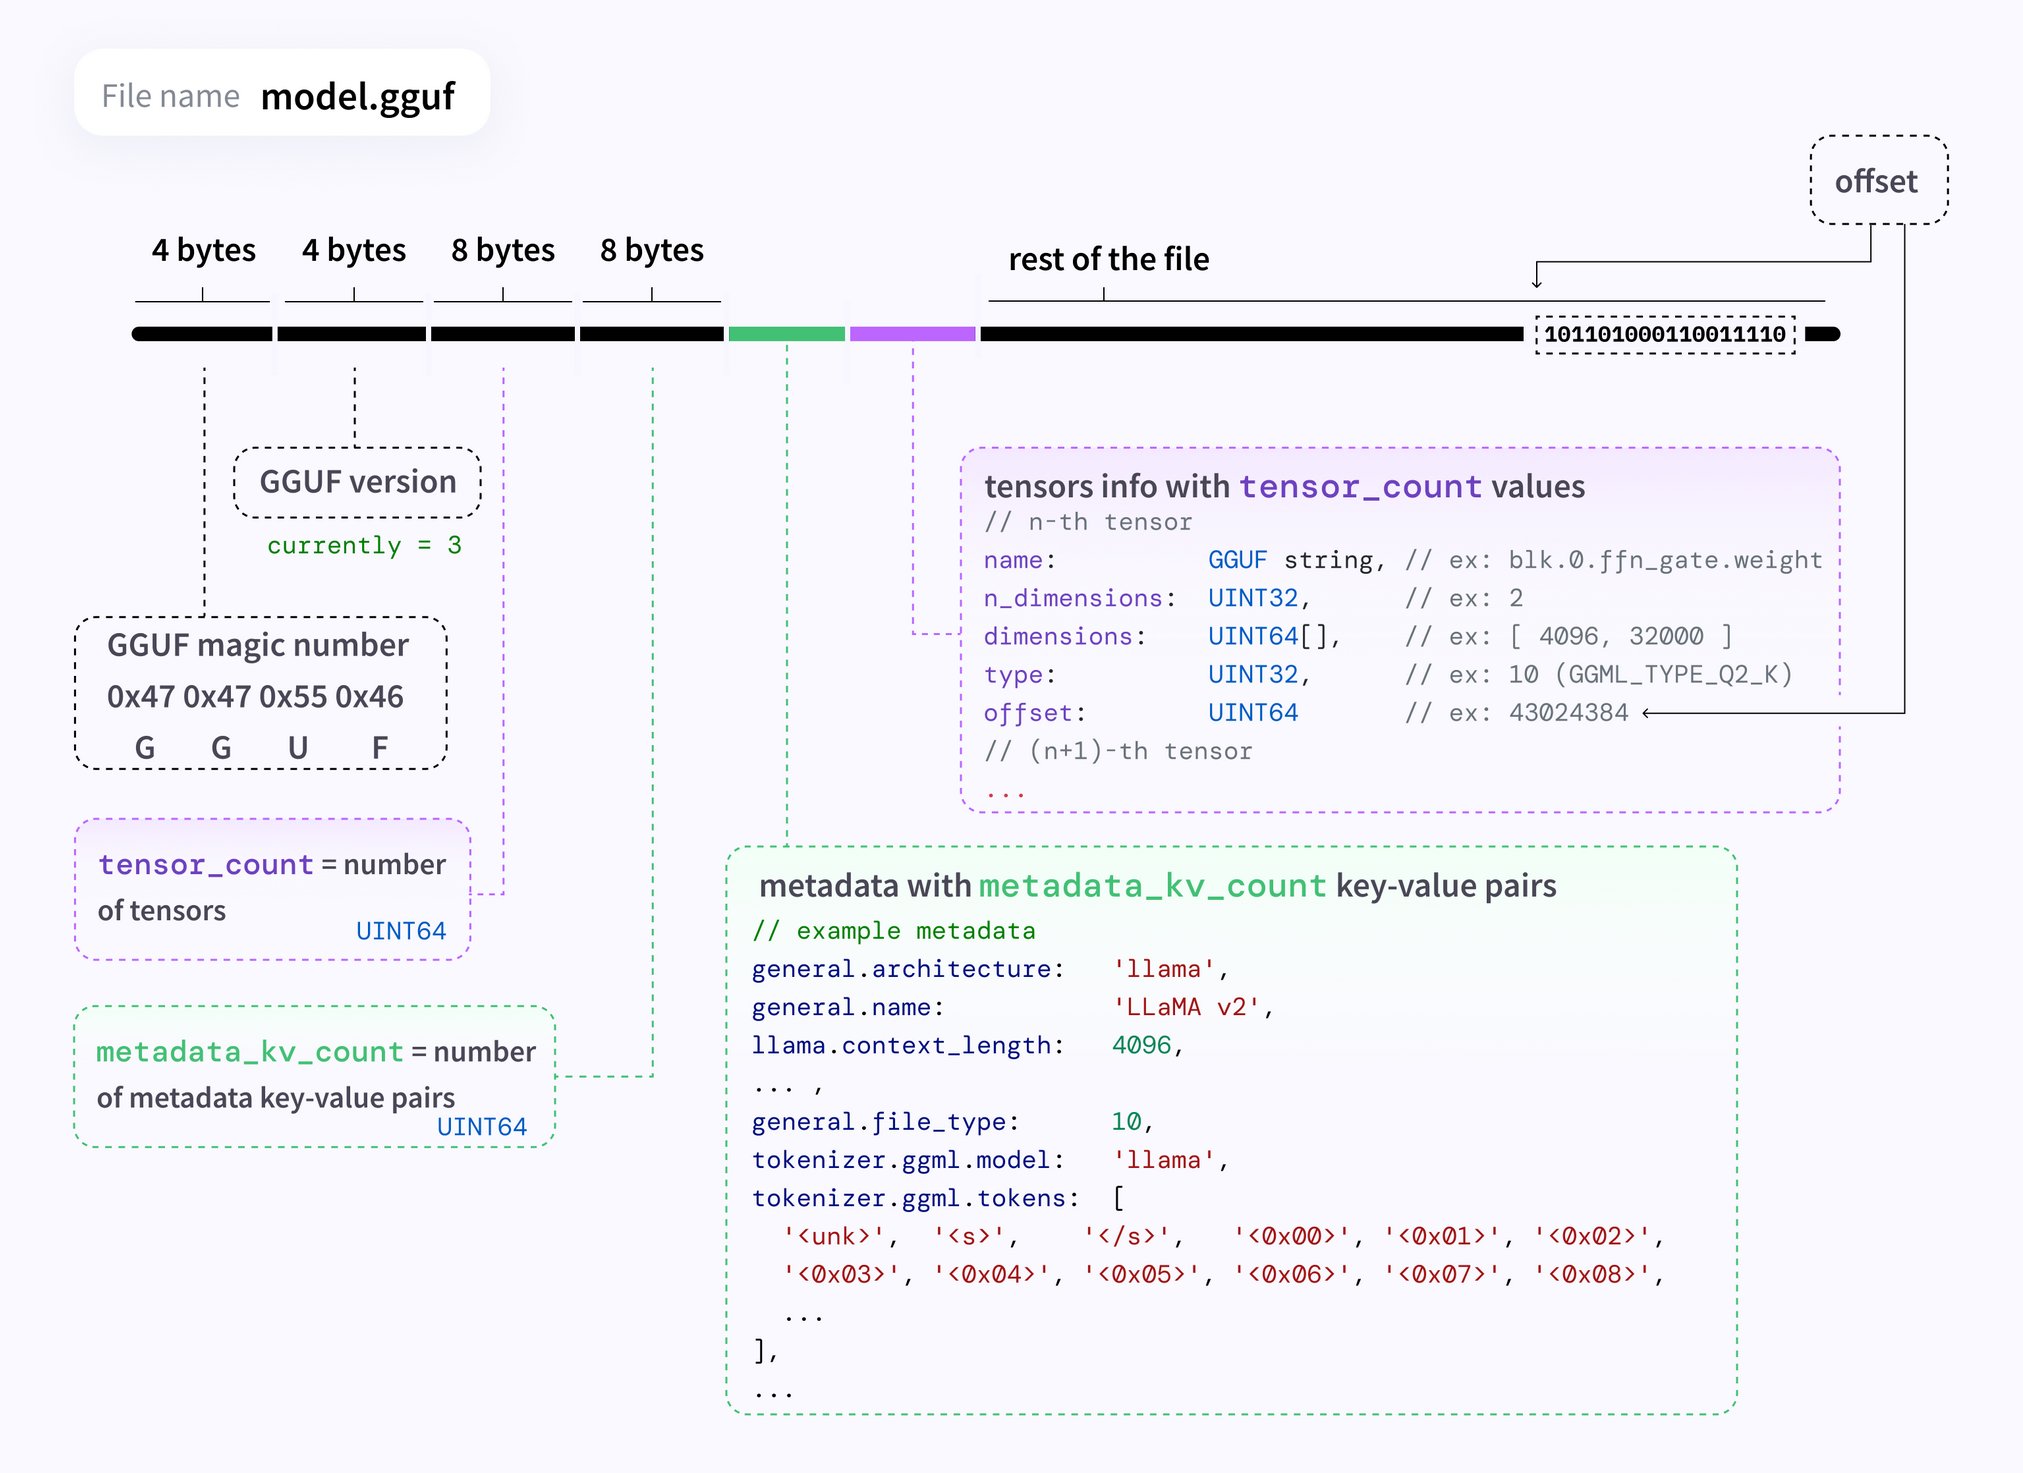
\includegraphics[height=0.5\textheight]{gguf}
			\captionof{figure}{GGUF Format Breakdown  (source:\cite{ggmlgithubdocs}).}
			\label{fig:gguf}
		\end{minipage}
	\end{strip}
	
	\begin{strip}
		\begin{minipage}{\textwidth}\centering
			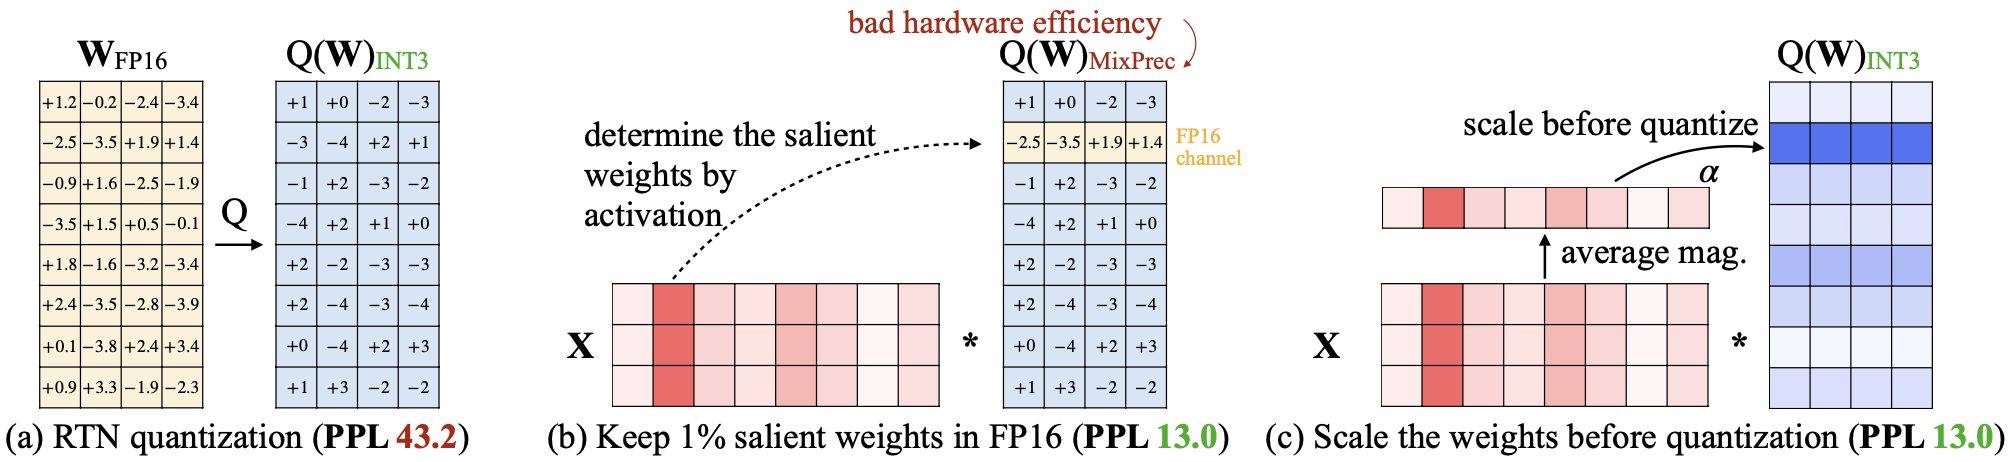
\includegraphics[height=0.15\textheight]{awq}
			\captionof{figure}{\gls{awq} method showing how scaling \textit{salient} weights before quantizations shows comparable results to mixed precision weights but without the hardware inefficiencies mix precision introduces (source:\cite{lin2024awqactivationawareweightquantization}).}
			\label{fig:awq}
		\end{minipage}
	\end{strip}
	
	The \texttt{llama.cpp} software developed by Georgi Gerganov and the open-source community is used to load the \gls{gguf} format. After it is loaded and processed based on the stored metadata, the underlying \gls{ggml} library can then begin inferencing the \gls{llm}~\cite{ggufgithub}. The \gls{gguf} format offers various quantization options, originally the quantization method was to simply split each layer into blocks of 256 weights and each block is then converted into their 256 quantized values, this was denoted with the letter \textbf{Q}. Additionally, there are two quantization type, ``type-0" (\textbf{Q4\_0}, \textbf{Q5\_0}, etc.) where weights $w$ are calculated from quants $q$ and block scale $d$ using $w = d \times q$. While ``type-1" (\textbf{Q4\_1}, \textbf{Q5\_1}, etc.) include an additional block minimum constant $m$ such that $w = d \times q + m$~\cite{ggufgithubquantdoc, ggufgithubkquantpr}. 
	
	Later the community have developed the \textbf{K} Quants, which expand the quantization range to include 2-bit, 3-bit and 6-bit quantization and prioritise certain weights over others (as denoted by suffixes like \textbf{Q3\_K\_S}, \textbf{Q3\_K\_M}, \textbf{Q3\_K\_L}) leading to smaller models with minimal \gls{ppl} increase~\cite{ggufgithubkquantpr}. The newest form of \gls{gguf} quants are the \textbf{I} quants, which add very low bit quantization capability~\cite{ggufgithubiquantpr} and are implemented based on the QuIP\# paper. According to this research paper, QuIP\# achieves low-bit quantization through clever groupings of quants. For instance, even numbers of either positive or negative signed values are grouped into 8 quants, allowing sign information to be recorded using only 7 bits. This, combined with the use of an E8 lattice structure, enables very low-bit quantization~\cite{tseng2024quipbetterllmquantization,ggufgithubiquantpr}. 
	
	
	\subsection{\gls{awq} \gls{ptq}}
	
	Similar to the \textbf{K} Quants of \gls{gguf}, the \gls{awq} method proposes a similar approach of selectively quantizing \gls{llm} weights depending on their importance by analysing the model activation patterns~\cite{lin2024awqactivationawareweightquantization}. This method identifies \textit{salient} weights in the \gls{llm} that hold more importance to the \gls{llm} performance and withhold quantization for those weights, thereby avoiding significant performance degradation when reducing the model size. However, having  mixed precision weights is not hardware-efficient, it was found that scaling the weights before quantization mitigates this issue while still preserving the benefits (see Figure \ref{fig:awq}).
	
	\subsection{\gls{vptq} \gls{ptq}}
	
	Similar to the \textbf{I} Quants of \gls{gguf}, the \gls{vptq} method is a low bit \gls{llm} quantization method that claims better accuracy for 1-2 bit \gls{llm} quantization compared to other conventional methods. It achieves this by compressing vectors into indices using lookup tables, with further refinement of weights using Channel-Independent Second-Order Optimization~\cite{liu2024vptqextremelowbitvector}. It differs from the previously covered \gls{awq} method as instead of reducing the precision of weights, it builds an index that maps high-dimensional vectors to lower-dimensional vectors. Figure \ref{fig:vptq} shows \gls{vptq} method achieves performance comparable to QuIP\#, the quantization technique that \gls{gguf}'s I-Quants are based on.
	
	\begin{figure}[h]
		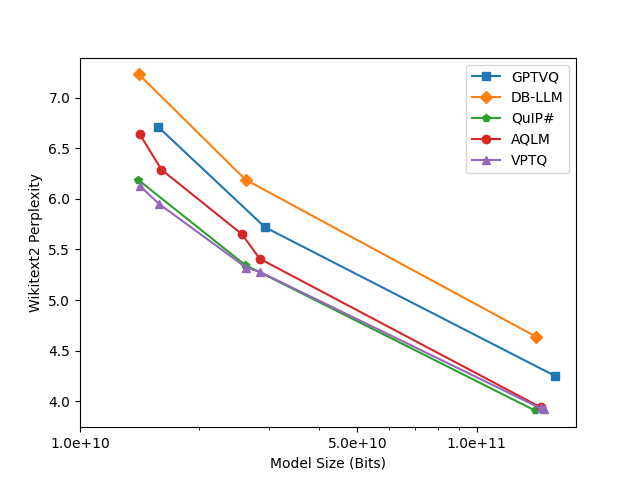
\includegraphics[width=1.1\linewidth]{vptq}
		\captionof{figure}{Graph showing \gls{ppl} of Wikitext2 dataset compared to model size using various \gls{ptq} methods (source:\cite{vptqgithub}).}
		\label{fig:vptq}
	\end{figure}
	
	\subsection{\gls{llm} Pruning}
	Model pruning is a way of compressing the size of a model by removing certain components from the model while avoiding severe damage to how the model functions. This is achieved by removing redundant or unimportant singular or groups of neurons~\cite{huang2024largelanguagemodelpruning}. There are two type of pruning methods that can be performed on a model, structured pruning and unstructured pruning, the former involves simplifying the model by removing entire structural weights such as channels or layers while maintaining the network structures, while the latter focuses on removing redundant neurons or links~\cite{huang2024largelanguagemodelpruning}. Between the two approaches, structured pruning has much better hardware compatibility compared to unstructured pruning which maybe require additional software or hardware treatment to complete the task~\cite{huang2024largelanguagemodelpruning}.
	
	LLM-Pruner is a tool developed to perform structural pruning on an \gls{llm} using gradient-based optimization processes for structure selection~\cite{ma2023llmprunerstructuralpruninglarge}. The LLM-Pruner uses an algorithm to detect dependencies within a model, this allows them to select optimal structured groups for pruning based on their importance estimation. Like with most pruning methods, a post pruning re-training is required, which can be called a ``recovery" phase, where it is trained on a small dataset in order to help maintain its performance~\cite{ma2023llmprunerstructuralpruninglarge}.
	
	Unlike LLM-Pruner, the Bonsai pruning method does not use a gradient-based structured pruning and is designed for more typical consumer grade hardware to execute~\cite{dery2024everybodyprunenowstructured}. It instead generates sub-models and evaluates their performance to give a more holistic view, which claim to outperform \gls{sota} ``gradient-based structured pruning methods like LLM-Pruner"~\cite[p.~2]{dery2024everybodyprunenowstructured} on 4/6 evaluation tests. Similar to LLM-Pruner, the Bonsai method performs post pruning operations to help recover some lost performance, but unlike LLM-Pruner, it uses distillation from the original model to the pruned model. However, in some cases this post pruning adaptation may not be necessary due to the robustness of the \gls{llm} as well as redundancy of its modules~\cite{dery2024everybodyprunenowstructured}.
	
	\subsection{\gls{llm} Benchmarking}
	
	There are many benchmark dataset available that are designed to test various capabilities of \glspl{llm}, and as mentioned in the research scope section, this research will focus on a subset of datasets from three categories of \textbf{General Knowledge and Language Understanding}, \textbf{Reasoning Capabilities}, \textbf{Truthfulness} and \textbf{Instruction Following}. Starting with \gls{mmlu} Pro dataset which is an iterative improvement over the original \gls{mmlu} dataset by removing trivial and noisy questions~\cite{wang2024mmluprorobustchallengingmultitask}. It is a dataset with a diverse fields such as mathematics, computer science, physics, chemistry, biology, business and more to produce over 12,000 questions~\cite{wang2024mmluprorobustchallengingmultitask}. The dataset is constructed as series of multiple choice questions with up to 10 possible response options, compared to only 4 in the original \gls{mmlu} dataset, which should reduce random guessing score~\cite{mmluprohuggingface}.
	
	Next dataset to look at is HellaSwag, which similar to \gls{mmlu} part of the \textbf{General Knowledge and Language Understanding} category. This dataset evaluates an \glspl{llm} capability of answering questions in a contextually appropriate and common-sense manner, referred to as \textit{common-sense natural language inference}~\cite{zellers2019hellaswagmachinereallyfinish}. Similar to \gls{mmlu} the dataset is structured as multiple choice questions.
	
	Moving onto the \textbf{Reasoning Capabilities} category, AGIEval dataset uses various human-centric exams to evaluate a models reasoning capabilities~\cite{zhong2023agievalhumancentricbenchmarkevaluating}. The dataset is constructed with a particular focus on human-level cognitive tasks and real-world scenarios following a wide range of exam papers like mathematics exams, lawyer qualification tests, college admission tests and other qualification exams~\cite[p.~5]{zhong2023agievalhumancentricbenchmarkevaluating}. The format of the dataset is comprised of multiple choice with an addition of some fill-in-the-blank questions that employ exact matching strategy during evaluation~\cite[p.~6]{zhong2023agievalhumancentricbenchmarkevaluating}.
	
	For the \textbf{Truthfulness} category there exists a TruthfulQA dataset that evaluates a model for providing accurate and unbiased information. The benchmark consists of over 800 questions that covers 38 categories which include law, health, finance, and politics~\cite{lin2022truthfulqameasuringmodelsmimic}. This dataset was designed to help address the concerns of accidental and/or malicious \gls{llm} misuse. It relies heavily on true or false questions and uses Wikipedia to source the factual information. The questions in the dataset were designed to be adversarial such that ``questions test a weakness to imitative false-hoods: false statements with high likelihood on the training distribution"~\cite[p.~4]{lin2022truthfulqameasuringmodelsmimic}
	
	Finally, for the \textbf{Instruction Following} there is the \gls{ifeval} dataset which was designed to evaluate how well a model follows a set of instructions in the prompt using verifiable instructions. A verifiable instruction is a specific, measurable and objective directive that, upon completion, can be checked and confirmed for adherence~\cite{zhou2023instructionfollowingevaluationlargelanguage}. The \gls{ifeval} has identified 25 types of verifiable instructions, with the dataset comprising 500 prompts based on these types. For example, an instruction prompt might ask an \gls{llm} to generate 25 sentences, the output of which can be automatically and objectively verified~\cite{zhou2023instructionfollowingevaluationlargelanguage}. This dataset is highly valuable as it evaluates a key \gls{llcompleteness m} capability: instruction following. This skill is crucial for performing well on multiple-choice questions, a common evaluation method in many other datasets. Additionally, these questions require structured responses for correct evaluation, making instruction-following a foundational skill in \gls{llm} evaluations.
	
	\subsection{Summary}
	This preliminary literature review section has explored some of the existing \gls{llm} \gls{ptq} methods such as \gls{gguf}, \gls{awq} and \gls{vptq}. All of the discussed methods operate based on similar principals of reducing the precision of the numeric values within the model weights. The \gls{gguf}, being a community driven open-source project has more options for quantization available to it in the form of \textbf{K} quants (which selectively quantize certain weights over others) and \textbf{I} quants. Following from this, the \gls{llm} pruning methods LLM-Pruner and Bonsai function by removing parts of the model which has little impact on its quality. The differing feature between the two approaches lies with its selection process for the structured groups (gradient-based versus sub-model evaluation). Finally, benchmarking review covered various datasets that evaluate specific model capabilities such as \textbf{General Knowledge and Language Understanding}, \textbf{Reasoning Capabilities}, \textbf{Truthfulness} and \textbf{Instruction Following}. 
	
	\section{Working Theory}
	Following from the preliminary literature review, this section will define \glspl{tp} based on the previously reviewed literature which will help guide this paper's \glspl{rq}.
	
	\textbf{\gls{tp}1}: \textit{The effectiveness of \gls{ptq} techniques in reducing computational requirements is influenced by the \gls{llm} architecture, where certain architectures benefit more than others}.\\
	Just like how the architecture of the model must be known in order to load it for inferencing, it must be known in order to perform \gls{ptq} operations. Given that there are many emerging architectures for \glspl{llm}, it stands to reason that some architectures would have greater support for quantization compared to others. For example, since Meta's LLaMa has a strong community following, it is reasonable to expect it would receive better support from the community compared to more obscure models.
	
	
	\textbf{\gls{tp}2}: \textit{The combination of \gls{ptq} and pruning can achieve significant reduction in hardware requirements compared to using only one approach over the other}.\\
	As covered earlier, quantization operates primary relies on reducing numerical precision of the models' weights, and does not alter the structural behaviour of the model, unlike pruning methods. Therefore, it is reasonable to consider that the two methods are non-mutually exclusive and in theory can be applied to the same model and thereby greatly reduce its hardware requirements. There has been limited research done on this to date, and it is an area worth exploring further, even if the effects end up being destructive.
	
	\textbf{\gls{tp}3}: \textit{The impacts of \gls{ptq} and pruning on \gls{llm} performance can vary across different types of tasks (i.e., Instruction Following, Knowledge)}.\\
	During \gls{llm} training, instruction following capabilities are fine-tuned on a base model, which has been trained solely to predict the next token in a sequence, unlike its ``knowledge" capabilities which would be instilled throughout the training process. Considering how non-uniform the training process is with respect to different \gls{llm} capabilities, it stands to reason that impacts of model compression techniques would not be distributed uniformly.
	
	
	\textbf{\gls{tp}4}: \textit{\glspl{llm} reasoning tasks will be more strongly impacted compared to knowledge retrieval tasks after applying a \gls{ptq} or pruning method}.\\
	Following from the previous \gls{tp}, reasoning tasks such as problem-solving and logical inference would require a model to be able to integrate information from multiple parts of its learned knowledge base, while knowledge retrieval is a more straightforward process. Given that model compression has some impact to quality, it is likely that reasoning related tasks would be more heavily impacted compared to knowledge retrieval tasks.
	
	
	\section{Research Design}
	\subsection{Introduction}
	This section will detail the methodology for determining the most effective method to reduce hardware requirement for running \glspl{llm}. The process will involve systematic evaluation and comparison of various compression methods described in this paper, applied to the \gls{selectedModels}. To evaluate various aspects of post-compression \glspl{llm}, the previously discussed benchmark tests will be used and compared to their pre-compression evaluations, thus demonstrating their feasibility and practicality in real-world applications.
	
	\subsection{Design}
	Initially, it is necessary to establish a baseline against which the experiments can be compared against. To do this, it is necessary to be able to run the unmodified \gls{selectedModels} and gather various metrics from it such as \gls{ppl}, \gls{tps} output speed and the results of the benchmark tests for all the categories. The \gls{llm} sampling parameters must be deterministic for all tests, this can be done by setting the temperature to 0 and top\_k to 1, additionally the seed should be kept constant for reproducibility. This must be done for all the \gls{selectedModels} recorded to be used as baseline for each model.
	
	After the baseline metrics have been recorded, each of the \gls{selectedModels} must be quantized using each of the \gls{selectedQuants}. Following this, like with the baseline metrics, the sampling parameters must be deterministic, and all the same metrics must be recalculated for the quantized models and recorded. For certain quantization method like \gls{vptq} which are new and have less community support, some coding might be required to support certain \gls{llm} architectures.
	
	After all metrics for the \gls{selectedQuants} have been recorded, the same process must be done for the pruning methods using LLM-Pruner and Bonsai, likewise setting deterministic sampling parameters.
	
	In order to satisfy \textbf{\gls{rq}1}, it's important to have a formula for scoring the models based on the gathered metrics. We can use the expected decrease in benchmark score to compare against the uncompressed model score. 
	
	$$
	D_i = \left(1 - \frac{B_i^c}{B_i^u}\right) \times 100
	$$
	$$
	D_{\text{overall}} = \frac{1}{n} \sum_{i=1}^{n} D_i
	$$
	
	Where $D_i$ is the percentage decrease in benchmark $i$ score of compressed model $B_i^c$ over uncompressed model $B_i^c$.
	
	Additionally, to get a singular quality score value for a model, we can use the following formula to combine the weighted benchmark scores, \gls{ppl} and \gls{tps}:
	
	$$
	Q = w_{B} \left( \sum_{i=1}^{n} w_i B_i \right) - w_{PPL} \left( PPL \right) + w_{TPS}(TPS) 
	$$
	
	Where $Q$ is the quality score of a model based on the weighted result of $n$ benchmarks, weighted \gls{ppl} and weighted \gls{tps}.
	
	Similarly, to satisfy \textbf{\gls{rq}2}, the same can be repeated for pruned models using the same formulas to compare uncompressed \glspl{llm} against their compressed counterpart.
	
	The final \textbf{\gls{rq}3}, will combine quantization and pruning methods. All the pruned models will undergo the same \gls{ptq} quantization as the uncompressed models and will be re-evaluated using the same benchmark tests to determine the effect of combining both compression methodologies on both the resulting size of the models as well as the qualities in relation to the uncompressed original models.
	
	\section{Research}
	\subsection{Establishing a Baseline for \gls{selectedModels}}
	In ordered to evaluate and demonstrate the effects of compression on a model, it is first necessary to establish a baseline to which we can compare the results. As covered in the previous sections, a set of recognized academic benchmark tests will be used to give us a baseline set of scores.
	
	Using \textit{lm-evaluation-harness}, a unified framework for testing \glspl{llm} on a large number of evaluation tasks \cite{eval-harness}, the benchmark tests \textbf{Hellaswag}, \textbf{AGIEval}, \textbf{TruthfulQA} and \textbf{IFEval} can be run in a consistent manner against our \gls{selectedModels}.
	
	\subsubsection{Setup}
	The installation, setup and usage of lm-evaluation-harness is documented on their Github page, which simply involves cloning the repository and installing the package by running \verb|pip install -e .| in the project root directory. This will install all necessary dependencies including the \verb|transformers| package, which would be necessary to run uncompressed full-precision models. Table \ref{baseline-scores} shows the baseline tested scores, from running \verb|lm_eval| commands as shown in Figure \ref{lm-eval-command}.
	
	\begin{figure}[H]
		\centering
		\begin{lstlisting}[language=bash,numbers=none]
			lm_eval --model hf \
			--model_args pretrained=google/gemma-2-9b-it \
			--tasks hellaswag,agieval,truthfulqa,ifeval \
			--device cuda:0 \
			--batch_size 1
		\end{lstlisting}
		\captionof{figure}{lm-evaluation-harness command for Gemma2-9B}
		\label{lm-eval-command}
	\end{figure}
	
	\begin{strip}
		\begin{minipage}{\textwidth}
			\centering
			\captionof{table}{Uncompressed Baseline Tested Scores and Official Scores}
			\begin{tabular}{|c|c|c|c|c|c|c|c|c|}
				\hline
				\multirow{2}{*}{\textbf{}} &
				\multicolumn{2}{c|}{\textbf{Gemma2-9B}} & \multicolumn{2}{c|}{\textbf{Llama3.1-8B}} & \multicolumn{2}{c|}{\textbf{Qwen2.5-7B}} \\
				\cline{2-7}& 
				Tested Score & Official Score &
				Tested Score & Official Score & 
				Tested Score & Official Score \\
				\hline
				\textbf{Hellaswag} & 81.05 & 81.9 & 79.17 & NA & 80.47 & 80.2 \\
				\hline
				\textbf{AGIEval} & 49.65 & 52.8 & 42.33 & 47.1 & 59.08  & NA \\
				\hline
				\textbf{TruthfulQA} & 60.18 & 50.27 & 54.04 & NA & 64.77 & 56.4 \\
				\hline
				\textbf{IFEval} & 76.02 & NA & 61.75 & 76.8 & 73.02 & 71.2 \\
				\hline
				\label{baseline-scores}
			\end{tabular}
			
			\begin{figure}[H]
				\centering
				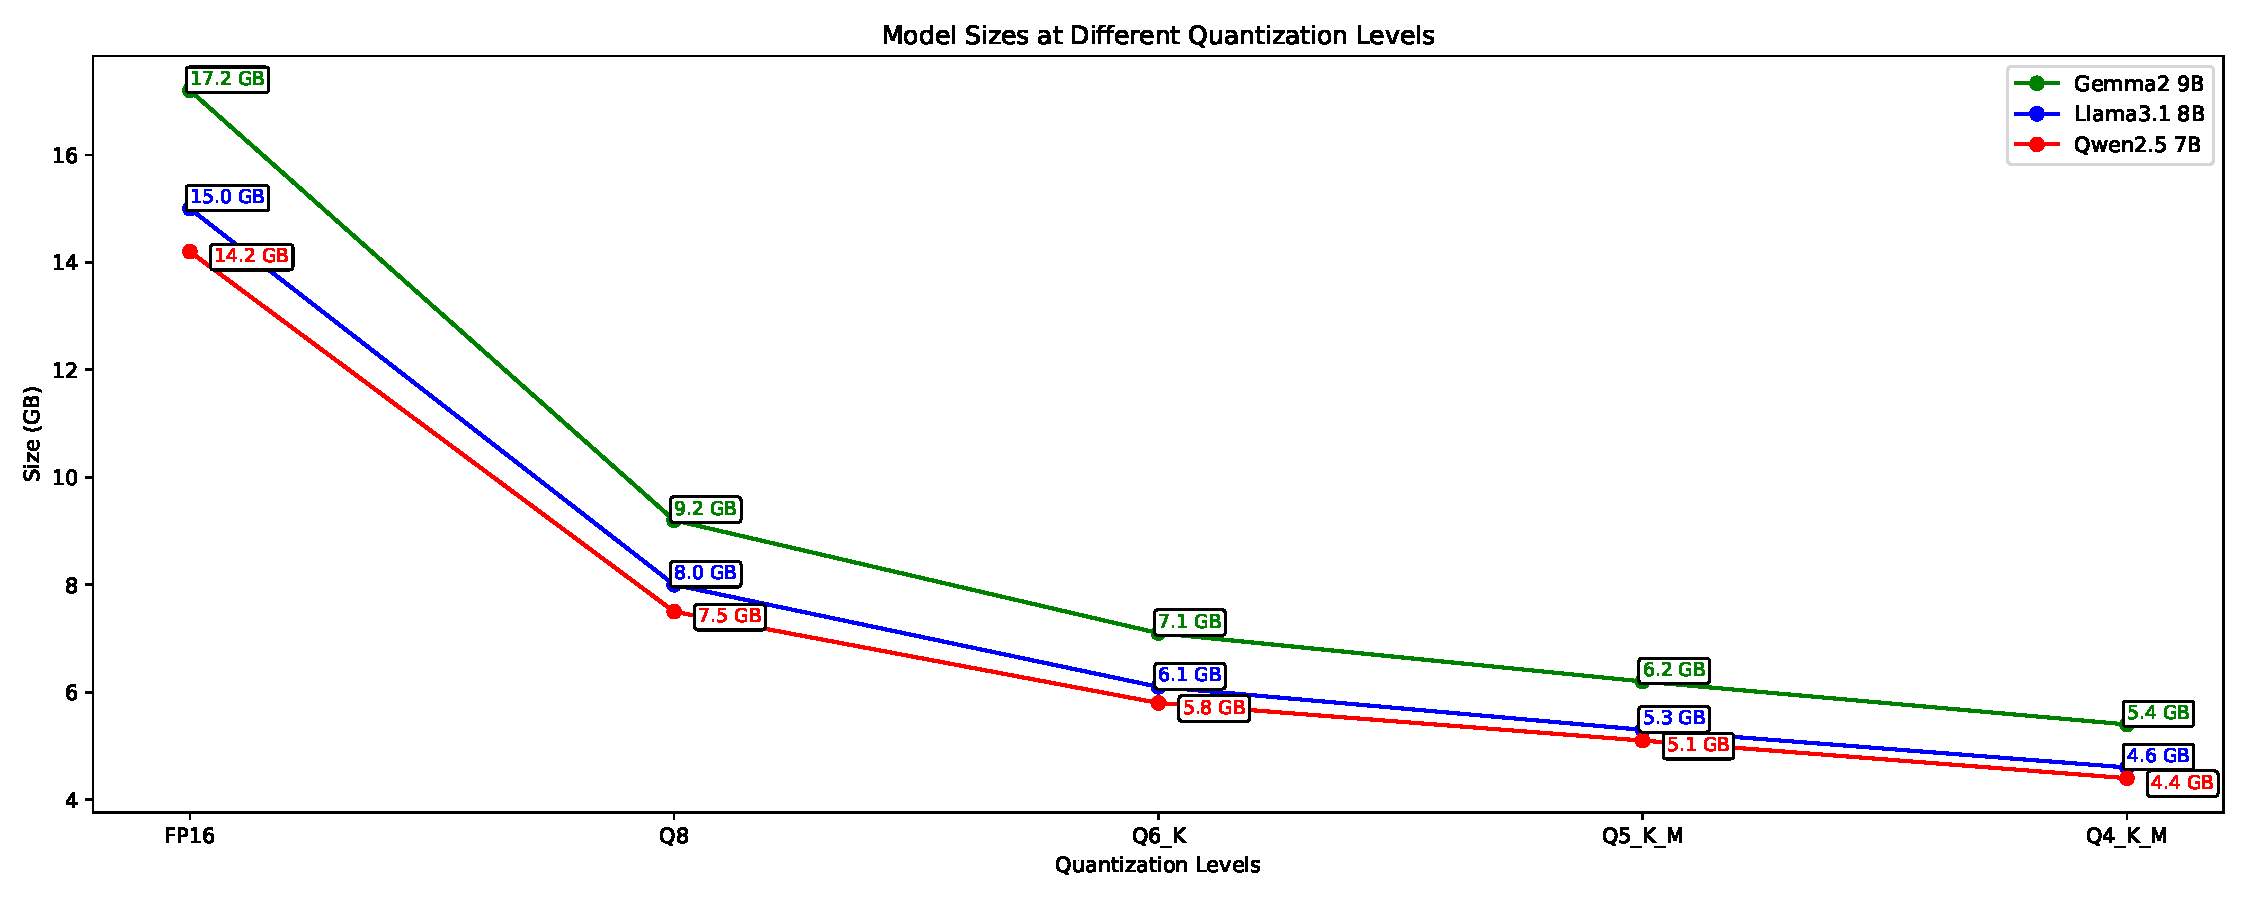
\includegraphics[width=\textwidth]{images/gguf-sizes.pdf}
				\label{fig:gguf-sizes}
			\end{figure}
			\captionof{figure}{\gls{gguf} Sizes}
		\end{minipage}
	\end{strip}
	
	\subsection{\gls{gguf} Quantization}
	\gls{gguf} quantization requires the Llama.cpp project \cite{llamacpp}. In order to quantize a model, it is first necessary to convert (i.e., package) the model into a \gls{gguf} format, which is achieved using the \verb|convert_hf_to_gguf.py| Python script within the LLamaCPP repository and produces a full precision FP16 \gls{gguf} model file.
	
	In order to quantize this \gls{gguf} file to a desired quant, it's necessary to compile LLamaCPP project using \verb|cmake|. The resulting binaries include \verb|llama-quantize| which is responsible for quantizing the full precision \gls{gguf} file outputted by the Python script earlier. 
	
	For I-Matrix quantization types, due to their very low precision, it's required to compute the importance matrix from the full precision model in order to determine important weights, this can be done using another compiled binary \verb|llama-imatrix| and training file (e.g., wiki.train.raw) which will be used for inferencing the model and identifying important weights. When quantizing a \gls{gguf} file with imatrix support, the output of \verb|llama-imatrix| must be supplied to ensure critical weights are preserved.
	
	\begin{figure}[H]
		\centering
		\begin{lstlisting}[language=bash,numbers=none]
			# Convert gemma2-9B-it model to GGUF format
			python convert_hf_to_gguf.py \
			--outfile Gemma2-GGUF/ gemma-2-9B-it/
			
			# Compile LLamaCPP binaries
			cmake -B build -DGGML_CUDA=ON
			cmake --build build --config Release -j 8
			
			# Compute importance matrix
			./llama.cpp/build/bin/llama-imatrix \
			-m Gemma2-GGUF/gemma-2-9B-it-F16.gguf \
			-f wikitext-2-raw/wiki.train.raw \
			-o Gemma2-GGUF/imatrix_gemma2.dat \
			--chunk 100 \
			--n-gpu-layers 99
			
			# Quantize to Q8
			./llama.cpp/build/bin/llama-quantize \
			./Gemma2-GGUF/gemma-2-9B-it-F16.gguf \
			./Gemma2-GGUF/gemma-2-9B-it-IQ1_S.gguf \
			IQ1_S
			
			# Quantize to IQ1_S
			./llama.cpp/build/bin/llama-quantize \
			--imatrix Gemma2-GGUF/imatrix_gemma2.dat \
			./Gemma2-GGUF/gemma-2-9B-it-F16.gguf \
			./Gemma2-GGUF/gemma-2-9B-it-IQ1_S.gguf \
			IQ1_S
		\end{lstlisting}
		\captionof{figure}{\gls{gguf} quantization command for Gemma2-9B}
		\label{gguf-command}
	\end{figure}
	
	For inferencing the quantized \gls{gguf} models, LLamaCPP project provides two binaries: a terminal utility \verb|llama-cli| and an OpenAI compliant API server \verb|llama-server|. However, neither tool offers optimal performance for benchmark workloads involving thousands of batched prompts. This is because LLamaCPP is primarily designed to accommodate diverse hardware configurations, rather than optimizing for production-like workloads where high parallel throughput is critical. To reduce the time required to execute all the benchmark tests, vLLM \cite{vllm} inference engine was used, which supports direct loading and execution of quantized \gls{gguf} models with it's V0 engine.
	
	\subsubsection{Gemma2-9B}
	This model features an architecture that differs significantly from the models commonly supported by inference engines by utilizing a sliding attention window. Consequently, initial attempts to load its quantized \gls{gguf} models in vLLM resulted in failure, requiring a custom patch (pull request 14766 \cite{vllm-pr-14766}) to enable proper loading. Table \ref{tab:geamm2_gguf_scores} reveals inconsistent performance for Hellaswag and IFEval benchmarks compared to it's uncompressed counterpart. This behavior suggests residual implementation issues in the engine.
	
	\begin{table}[H]
		\centering
		\caption{Gemma2-9B \gls{gguf} Scores}
		\begin{tabular}{|>{\centering\arraybackslash}m{1.8cm}|*{4}{>{\centering\arraybackslash}m{1.2cm}|}}
			\hline
			\textbf{Benchmark Test} & \textbf{Q8} & \textbf{Q6\_K} & \textbf{Q5\_K\_M} & \textbf{Q4\_K\_M}  \\
			\hline
			Hellaswag & 65.45 & 65.21 & 65.08 & 64.79 \\
			\hline
			AGIEval & - & - & - & - \\
			\hline
			TruthfulQA & 62.25 & 62.15 & 62.07& 62.37 \\
			\hline
			IFEval & 34.41 & 35.49 & 35.61 & 35.97 \\
			\hline
		\end{tabular}
		\label{tab:geamm2_gguf_scores}
	\end{table}
	
	\subsubsection{Llama3.1-8B}
	Llama3.1-8B demonstrates the benefits of strong community support, being from a family of one of the earliest open-weight models, shows consistent performance across quantization levels (see Table \ref{tab:llama3.1_gguf_scores}). Unlike Gemma2-9B, it shows predictable degradation across all the benchmark scores.
	
	\begin{table}[H] % Use the H option to force the table to appear here
		\centering
		\caption{Llama3.1-8B \gls{gguf} Scores}
		\begin{tabular}{|>{\centering\arraybackslash}m{1.8cm}|*{4}{>{\centering\arraybackslash}m{1.2cm}|}}
			\hline
			\textbf{Benchmark Test} & \textbf{Q8} & \textbf{Q6\_K} & \textbf{Q5\_K\_M} & \textbf{Q4\_K\_M}  \\
			\hline
			Hellaswag & 79.19 & 79.09 & 78.99 & 78.74 \\
			\hline
			AGIEval & - & - & - & - \\
			\hline
			TruthfulQA & 54.01 & 53.78 & 53.37 & 52.56 \\
			\hline
			IFEval & 59.95 & 59.83 & 59.59 & 56.35 \\
			\hline
		\end{tabular}
		\label{tab:llama3.1_gguf_scores}
	\end{table}
	
	\subsubsection{Qwen2.5-7B}
	Qwen2.5-7B exhibits performance stability comparable to Llama3.1-8B (Table \ref{tab:qwen2.5_gguf_scores}), reflecting its strong community adoption. The results, which are consistent with Llama3.1-8B, validates that community-supported models achieve reliable quantization outcomes, contrasting sharply with Gemma's implementation challenges.
	
	\begin{table}[H] 
		\centering
		\caption{Qwen2.5-7B \gls{gguf} Scores}
		\begin{tabular}{|>{\centering\arraybackslash}m{1.8cm}|*{4}{>{\centering\arraybackslash}m{1.2cm}|}}
			\hline
			\textbf{Benchmark Test} & \textbf{Q8} & \textbf{Q6\_K} & \textbf{Q5\_K\_M} & \textbf{Q4\_K\_M}  \\
			\hline
			Hellaswag & 80.46 & 80.34 & 80.37 & 80.19 \\
			\hline
			AGIEval & - & - & - & - \\
			\hline
			TruthfulQA & 64.72 & 65.23 & 65.37 & 64.28 \\
			\hline
			IFEval & 71.34 & 73.50 & 71.10 & 71.46 \\
			\hline
		\end{tabular}
		\label{tab:qwen2.5_gguf_scores}
	\end{table}
	\newpage
	
	\subsection{AWQ Quantization}
	To quantize the \gls{selectedModels} using \gls{awq} method, the vLLM project provides the llm-compressor library \cite{lllm-compressor}, which integrates the AutoAWQ quantization framework. While this tool enables \gls{awq} quantization of our models, the process requires significantly higher VRAM than \gls{gguf} quantization. Given the hardware constraints, it was not possible to directly quantize the models using AutoAWQ, and instead the approach adopted was to source them from the open source community on \url{huggingface.co}, which hosts community-verified \gls{selectedModels} quantized with \gls{awq}. For completeness, the script necessary to quantize using \gls{awq} is provided in Figure \ref{awq-script}.
	
	\begin{figure}[H]
		\centering
		\begin{lstlisting}[language=python,numbers=none]
			import argparse
			from llmcompressor.modifiers.awq import AWQModifier
			from llmcompressor import oneshot
			
			def main(model_path, output_dir):
			# Define the quantization recipe using AWQ
			recipe = [
			AWQModifier(ignore=["lm_head"], scheme="W4A16_ASYM", targets=["Linear"]),
			]
			
			# Apply quantization using the specified model path and output directory
			oneshot(
			model=model_path,
			recipe=recipe,
			dataset="open_platypus",
			output_dir=output_dir,
			max_seq_length=2048,
			num_calibration_samples=512,
			)
			
			if __name__ == "__main__":
			# Set up argument parsing
			parser = argparse.ArgumentParser(description="Quantize an LLM model using AWQ.")
			parser.add_argument("--model_path", type=str, required=True, help="Path to the local model directory.")
			parser.add_argument("--output_dir", type=str, required=True, help="Directory to save the quantized model.")
			
			# Parse the arguments
			args = parser.parse_args()
			
			# Call the main function with the parsed arguments
			main(args.model_path, args.output_dir)
			
		\end{lstlisting}
		\captionof{figure}{\gls{awq} quantization python script using AutoAWQ from llm-compressor library}
		\label{awq-script}
	\end{figure}
	
	\begin{table}[H]
		\centering
		\captionof{table}{\gls{awq} Benchmark Results}
		\begin{tabular}{|l|c|c|c|}
			\hline
			\multirow{1}{*}{\textbf{Benchmark}} & \textbf{Gemma2-9B} & \textbf{Llama3.1-8B} & \textbf{Qwen2.5-7B} \\ \hline
			\textbf{Hellaswag}                & 63.47            & 78.49              & 79.57              \\ \hline
			\textbf{AGIEval}                  & -            & -              & -              \\ \hline
			\textbf{TruthfulQA}               & 61.86            & 42.99              & 63.77              \\ \hline
			\textbf{IFEval}                   & 31.77            & 64.47              & 69.78              \\ \hline
		\end{tabular}
		\label{tab:awq_results}
	\end{table}
	
	The results of the benchmark tests which ran against \gls{awq} quantized models can be seen in Table \ref{tab:awq_results}. From this, we can already draw some parallels to the previous benchmark results from \gls{gguf} models earlier. Specifically, once again Gemma2-9B suffers noticeable and non trivial drops in performance compared to uncompressed results. While from a broad general viewpoint, it appears that all three models score worse than the \textbf{Q4\_K\_M} \gls{gguf} counterparts on the same benchmark tests.
	
	\subsection{\gls{vptq} Quantization}
	Similar to \gls{awq}, \gls{vptq} quantization requires signifant resources to successfully compress the original model, therefore, like with the previous method, the models were downloaded from \url{huggingface.co}. Unfortunately, the Gemma2-9B model has not been quantized by the community using \gls{vptq} at the time of this investigation and only the Llama3.1-8B and Qwen2.5-7B models were available. Unlike \gls{awq}, \gls{vptq} does not yet have widespread support in various inferencing engines, but fortunately support for \gls{vptq} has been merged into the Transformers library, and therefore can be directly used by \textit{lm-evaluation-harness} without relying on vLLM.
	
	\begin{table}[H]
		\centering
		\captionof{table}{\gls{vptq} Benchmark Results}
		\begin{tabular}{|l|c|c|c|}
			\hline
			\multirow{1}{*}{\textbf{Benchmark}} & \textbf{Gemma2-9B} & \textbf{Llama3.1-8B} & \textbf{Qwen2.5-7B}  \\ \hline
			\textbf{Hellaswag}                & -            & 76.07              & 78.17              \\ \hline
			\textbf{AGIEval}                  & -            & -              & -              \\ \hline
			\textbf{TruthfulQA}               & -            & 49.60              & 61.84              \\ \hline
			\textbf{IFEval}                   & -            & 59.95              & 71.70              \\ \hline
		\end{tabular}
		\label{tab:vptq_results}
	\end{table}
	
	The results of the benchmark tests for \gls{vptq} models can be seen in Table \ref{tab:vptq_results}. Comparing \gls{vptq} results to \gls{awq} above, it appears that there is an overall degradation in scores except for \textbf{TruthfulQA} for Llama3.1-8B and \textbf{IFEval} for Qwen2.5-7B. The former having a much greater difference between the two compression methods.
	\newpage
	
	\subsection{Quantization Conclusion}
	\begin{strip}
		\begin{minipage}{\textwidth}
			\centering
			\captionof{table}{Quantization Benchmark Scores and Sizes}
			\label{tab:gguf_combined_results}
			\begin{tabular}{|l|*{3}{>{\centering\arraybackslash}m{2.4cm}|}>{\centering\arraybackslash}m{2.4cm}|*{3}{>{\centering\arraybackslash}m{2cm}|}}
				\hline
				\multirow{2}{*}{\textbf{Model}} & \multirow{2}{*}{\textbf{Compression}} & \multirow{2}{*}{\textbf{Size}} & \multicolumn{4}{c|}{\textbf{Benchmark Scores}} \\
				\cline{4-7}
				& & & \textbf{Hellaswag} & \textbf{AGIEval} & \textbf{TruthfulQA} & \textbf{IFEval} \\
				\hline
				\multirow{7}{*}{Gemma2-9B}
				& BF16 & 17.2 GB & 81.05 & 49.65 & 60.18 & 76.02 \\
				& Q8 & 9.2 GB & 65.45 & - & 62.25 & 34.41 \\
				& Q6\_K & 7.1 GB & 65.21 & - & 62.15 & 35.49 \\
				& Q5\_K\_M & 6.2 GB & 65.08 & - & 62.07 & 35.61 \\
				& Q4\_K\_M & 5.4 GB & 64.79 & - & 62.37 & 35.97 \\
				& AWQ & 5.8 GB & 63.47 & - & 61.86 & 31.77 \\
				& VPTQ & - & - & - & - & - \\
				\hline
				\multirow{7}{*}{Llama3.1-8B}
				& BF16 & 15.0 GB & 79.17 & 42.33 & 54.04 & 61.75 \\
				& Q8 & 8.0 GB & 79.19 & - & 54.01 & 59.95 \\
				& Q6\_K & 6.1 GB & 79.09 & - & 53.78 & 59.83 \\
				& Q5\_K\_M & 5.3 GB & 78.99 & - & 53.37 & 59.59 \\
				& Q4\_K\_M & 4.6 GB & 78.74 & - & 52.56 & 56.35 \\
				& AWQ & 5.4 GB & 78.49 & - & 42.99 & 64.47 \\
				& VPTQ & 4.6 GB & 76.07 & - & 49.60 & 59.95 \\
				\hline
				\multirow{7}{*}{Qwen2.5-7B}
				& BF16 & 14.2 GB & 80.47 & 59.08 & 64.77 & 73.02 \\
				& Q8 & 7.5 GB & 80.46 & - & 64.72 & 71.34 \\
				& Q6\_K & 5.8 GB & 80.34 & - & 65.23 & 73.50 \\
				& Q5\_K\_M & 5.1 GB & 80.37 & - & 65.37 & 71.10 \\
				& Q4\_K\_M & 4.4 GB & 80.19 & - & 64.28 & 71.46 \\
				& AWQ & 5.2 GB & 79.57 & - & 63.77 & 69.78 \\
				& VPTQ & 4.5 GB & 78.17 & - & 61.84 & 71.70 \\
				\hline
			\end{tabular}
			\begin{table}[H]
				\centering
				\captionof{table}{Pruning Benchmark Results}
				\begin{tabular}{|l|c|c|c|}
					\hline
					\textbf{Benchmark} & \textbf{Gemma2-9B (Pruned)} & \textbf{Llama3.1-8B (Pruned)} & \textbf{Qwen2.5-7B (Pruned)} \\ \hline
					\textbf{Hellaswag}                & 53.93 & 71.03 & 49.67 \\ \hline
					\textbf{AGIEval}                  & -     & -     & -     \\ \hline
					\textbf{TruthfulQA}               & 43.34 & 46.14 & 51.58 \\ \hline
					\textbf{IFEval}                   & 30.82 & 14.75 & 27.46 \\ \hline
					\textbf{Original Size (GB)}        & 17.2  & 15.0  & 14.2  \\ \hline
					\textbf{Pruned Size (GB)}          & 12.2  & 13.0  & 9.1   \\ \hline
					\textbf{Size Reduction vs Uncompressed (\%)} & 29.1\% & 13.3\% & 35.9\% \\ \hline
				\end{tabular}
				\label{tab:pruning_results}
			\end{table}
		\end{minipage}
	\end{strip}
	
	Table \ref{tab:gguf_combined_results} combines the results of the benchmark tests for all of the \gls{selectedModels}, showcasing the size reductions for each quantization as well as the associated benchmark scores. A notable highlight from the table is the Gemma2-9B model, unlike its TruthfulQA score, the IFEval and Hellaswag were both negatively affected by quantization unlike the other two models. This could probably be attributed to the lack of proper inference engine support for the model itself, as mentioned in the previous section.
	
	\subsection{Pruning}
	In the process of conducting this research, it was discovered that the hardware requirements necessary to prune any of the \gls{selectedModels} significantly exceed the allocated hardware resourced for this research, specified in section 1.3 Research Scope and Limitations. Using a different \gls{llm} model outside of the established \gls{selectedModels}, Llama3.2-3B which is sized at 5.5GB uncompressed. It was discovered that pruning for such as model required almost 18GB of VRAM. Therefore, using the compute hardware allocated for this research would be insufficient to prune the \gls{selectedModels}.
	
	As such, pre-pruned models were used for this evaluation. The parameters and conditions under which these models were pruned is not known, as such, it is not possible to evaluate all pruning configurations. 
	The pruned Gemma2-9B was sourced from \url{https://huggingface.co/Arrebol-logos/Pruned-Once-Gemma2-9B}, the pruned LLaMa 3.1-8B was sourced from \url{https://huggingface.co/Na0s/Llama-3.1-8B-Pruned-4-Layers} and finally the pruned Qwen2.5-7B was sourced from \url{https://huggingface.co/Aarushhh/Qwen-2.5-7b-Instruct-Pruned}.
	
	
	Table \ref{tab:pruning_results} shows the results benchmark scores for the pruned models. While the size reduction relative to the original models is significant, the models scored significantly lower than even the most aggressive \gls{ptq} quantization method. Particularly, the IFEval benchmark, which measures the models instruction following capabilities, suffers substantially from undergoing pruning. Furthermore, while the pruned model's resize reduction is significant, it is still lower than what can be achieve with \textbf{Q8} \gls{gguf} quantization, which is also one of the least aggressive quantization and therefore should preserve the most quality of the model.
	
	\vfill
	\clearpage
	\pagebreak
	
	\subsection{Pruned Model Quantization}
	\begin{strip}
		\begin{minipage}{\textwidth}
			\begin{table}[H]
				\centering
				\captionof{table}{Gemma2-9B}
				\begin{tabular}{|l|c|c|c|c|}
					\hline
					\textbf{Benchmark} & \textbf{Q8 (Pruned)} & \textbf{Q6\_K (Pruned)} & \textbf{Q5\_K\_M (Pruned)} & \textbf{Q4\_K\_M (Pruned)} \\ \hline
					\textbf{Hellaswag} & 30.82 & 30.94 & 25.04 & 25.04 \\ \hline
					\textbf{IFEval}    & 35.97 & 34.77 & 35.85 & 24.82 \\ \hline
					\textbf{TruthfulQA} & 46.70 & 47.10 & 46.55 & 45.59 \\ \hline
					\textbf{Size (GB)} & 5.6 & 4.5 & 3.9 & 3.5 \\ \hline
					\textbf{Reduction vs Uncompressed (\%)} & 67.4\% & 73.8\% & 77.4\% & 79.7\% \\ \hline
				\end{tabular}
				\label{tab:gemma_pruned_quantized}
			\end{table}
			
			\begin{table}[H]
				\centering
				\captionof{table}{Llama3.1-8B}
				\begin{tabular}{|l|c|c|c|c|}
					\hline
					\textbf{Benchmark} & \textbf{Q8 (Pruned)} & \textbf{Q6\_K (Pruned)} & \textbf{Q5\_K\_M (Pruned)} & \textbf{Q4\_K\_M (Pruned)} \\ \hline
					\textbf{Hellaswag} & 71.05 & 70.98 & 70.77 & 70.79 \\ \hline
					\textbf{IFEval}    & 16.31 & 15.95 & 16.07 & 17.39 \\ \hline
					\textbf{TruthfulQA} & 46.17 & 46.32 & 46.02 & 46.49 \\ \hline
					\textbf{Size (GB)} & 6.9 & 5.3 & 4.6 & 4.0 \\ \hline
					\textbf{Reduction vs Uncompressed(\%)} & 54.0\% & 64.7\% & 69.7\% & 73.3\% \\ \hline
				\end{tabular}
				\label{tab:llama_pruned_quantized}
			\end{table}
			
			\begin{table}[H]
				\centering
				\captionof{table}{Qwen2.5-7B}
				\begin{tabular}{|l|c|c|c|c|}
					\hline
					\textbf{Benchmark} & \textbf{Q8 (Pruned)} & \textbf{Q6\_K (Pruned)} & \textbf{Q5\_K\_M (Pruned)} & \textbf{Q4\_K\_M (Pruned)} \\ \hline
					\textbf{Hellaswag} & 27.73 & 27.71 & 25.04 & 27.60 \\ \hline
					\textbf{IFEval}    & 26.86 & 26.26 & 25.78 & 26.62 \\ \hline
					\textbf{TruthfulQA} & 49.31 & 49.28 & 49.25 & 49.22 \\ \hline
					\textbf{Size (GB)} & 4.9 & 4.0 & 3.4 & 3.0 \\ \hline
					\textbf{Reduction vs Uncompressed(\%)} & 65.5\% & 71.8\% & 76.1\% & 78.9\% \\ \hline
				\end{tabular}
				\label{tab:qwen_pruned_quantized}
			\end{table}
		\end{minipage}
	\end{strip}
	
	The process of quantizing the pruned models follows the same procedure as quantizing the uncompressed original models. Tables \ref{tab:gemma_pruned_quantized}, \ref{tab:llama_pruned_quantized}, and \ref{tab:qwen_pruned_quantized} demonstrate significant size reductions compared to their uncompressed counterparts, with the Q4\_K\_M achieving smaller sizes than \gls{vptq}. However, this significant size reduction comes at a substantial performance cost: as expected, benchmark scores deteriorate with increased quantization levels. Notably, while IFEval performance degrades severely for most models, Llama3.1-8B showed unexpected recovery compared to its pruned-unquantized counterpart. Most surprisingly, Gemma2-9B experienced minimal IFEval degradation.
	
	\subsection{Calculating \gls{ppl}}
	\gls{ppl} measures how well a model predicts the next token during text generation, with lower values indicating better performance. However, because different models use different tokenizers, \gls{ppl} scores aren't directly comparable across models but are still a valuable metric for evaluating the affects of compression. To ensure consistency in \gls{ppl} computation across models, this analysis exclusively uses \gls{gguf}, which provides standardized evaluation tools (e.g., \verb|llama-perplexity)|). Following LLamaCPP convention, Wikitext-2 test set was used for testing perplexity with this tool.
	
	\begin{table}[H]
		\centering
		\captionof{table}{Gemma2-9B PPL Results}
		\begin{tabular}{|l|c|c|}
			\hline
			\textbf{Quantization} & \textbf{PPL (Original)} & \textbf{PPL (Pruned)} \\ \hline
			F16 & 8.7895 (±0.06502) & 20.0294 (±0.15731) \\ \hline
			Q8 & 8.7841 (±0.06495) & 20.0364 (±0.15743) \\ \hline
			Q6\_K & 8.7960 (±0.06508) & 20.0772 (±0.15776) \\ \hline
			Q5\_K\_M & 8.7876 (±0.06497) & 20.2195 (±0.15932) \\ \hline
			Q4\_K\_M & 8.8984 (±0.06601) & 20.5338 (±0.16168) \\ \hline
		\end{tabular}
		\label{tab:gemma_ppl}
	\end{table}
	
	\begin{table}[H]
		\centering
		\captionof{table}{Llama3.1-8B PPL Results}
		\begin{tabular}{|l|c|c|}
			\hline
			\textbf{Quantization} & \textbf{PPL (Original)} & \textbf{PPL (Pruned)} \\ \hline
			F16 & 7.3257 (±0.04676) & 19.8279 (±0.15175) \\ \hline
			Q8 & 7.3281 (±0.04677) & 19.8173 (±0.15164) \\ \hline
			Q6\_K & 7.3541 (±0.04699) & 19.7985 (±0.15162) \\ \hline
			Q5\_K\_M & 7.3985 (±0.04730) & 20.1740 (±0.15479) \\ \hline
			Q4\_K\_M & 7.5316 (±0.04814) & 20.4621 (±0.15667) \\ \hline
		\end{tabular}
		\label{tab:llama_ppl}
	\end{table}
	
	\begin{table}[H]
		\centering
		\captionof{table}{Qwen2.5-7B PPL Results}
		\begin{tabular}{|l|c|c|}
			\hline
			\textbf{Quantization} & \textbf{PPL (Original)} & \textbf{PPL (Pruned)} \\ \hline
			F16 & 7.8932 (±0.05600) & 53.4464 (±0.52670) \\ \hline
			Q8 & 7.8999 (±0.05615) & 53.4556 (±0.52668) \\ \hline
			Q6\_K & 7.9020 (±0.05608) & 53.5285 (±0.52712) \\ \hline
			Q5\_K\_M & 7.9762 (±0.05687) & 53.9359 (±0.53118) \\ \hline
			Q4\_K\_M & 8.0541 (±0.05739) & 54.4885 (±0.53958) \\ \hline
		\end{tabular}
		\label{tab:qwen_ppl}
	\end{table}
	
	Tables \ref{tab:gemma_ppl}, \ref{tab:llama_ppl}, and \ref{tab:qwen_ppl} demonstrate a clear, progressive increase in \gls{ppl} with each step of quantization across all models, confirming the expected trade-off between compression and performance. More significantly, the unquantized pruned models already exhibit substantially higher \gls{ppl} scores compared to their original unpruned counterparts. This indicates that pruning substantially increases \gls{ppl}. However, as the exact pruning parameters and configurations of these models are unknown, we can only conclude that these specific pruned models show large disparity in \gls{ppl} scores compared to their original counterparts.
	
	\subsection{Calculating \gls{tps}}
	\gls{tps} measures the rate at which the model generates text during inference, with higher values indicating better throughput. Similar to the previous section, for consistency the \gls{gguf} models will be used and the \gls{tps} will be evaluated using the LLamaCPP tool \verb|llama-bench|. In order to ensure the evaluation was fair, each model was run three times using \verb|llama-bench| tool and generated 128, 256, and 512 output tokens respectively, the results of which were averaged.
	
	\begin{table}[H]
		\centering
		\captionof{table}{Gemma2-9B TPS Results}
		\begin{tabular}{|l|c|c|}
			\hline
			\textbf{Quantization} & \textbf{Original} & \textbf{Pruned} \\ \hline
			F16 & 44.09 (±0.30) & 68.05 (±0.11) \\ \hline
			Q8\_0 & 74.26 (±0.47) & 107.42 (±0.11) \\ \hline
			Q6\_K & 89.86 (±0.12) & 122.61 (±0.19) \\ \hline
			Q5\_K\_M & 99.41 (±0.07) & 134.89 (±0.18) \\ \hline
			Q4\_K\_M & 109.74 (±0.15) & 145.07 (±0.23) \\ \hline
		\end{tabular}
		\label{tab:gemma_tps}
	\end{table}
	
	\begin{table}[H]
		\centering
		\captionof{table}{Llama3.1-8B TPS Results}
		\begin{tabular}{|l|c|c|}
			\hline
			\textbf{Quantization} & \textbf{Original} & \textbf{Pruned} \\ \hline
			F16 & 56.61 (±0.07) & 66.23 (±0.12) \\ \hline
			Q8\_0 & 96.84 (±0.08) & 113.35 (±0.11) \\ \hline
			Q6\_K & 118.59 (±0.18) & 138.89 (±0.16) \\ \hline
			Q5\_K\_M & 131.83 (±0.35) & 154.36 (±0.17) \\ \hline
			Q4\_K\_M & 147.92 (±0.31) & 173.14 (±0.21) \\ \hline
		\end{tabular}
		\label{tab:llama_tps}
	\end{table}
	
	\begin{table}[H]
		\centering
		\captionof{table}{Qwen2.5-7B TPS Results}
		\begin{tabular}{|l|c|c|}
			\hline
			\textbf{Quantization} & \textbf{Original} & \textbf{Pruned} \\ \hline
			F16 & 59.97 (±0.10) & 92.69 (±0.27) \\ \hline
			Q8\_0 & 102.13 (±0.04) & 151.44 (±0.34) \\ \hline
			Q6\_K & 124.87 (±0.14) & 173.92 (±0.19) \\ \hline
			Q5\_K\_M & 139.25 (±0.54) & 194.58 (±0.87) \\ \hline
			Q4\_K\_M & 155.63 (±0.09) & 211.19 (±0.37) \\ \hline
		\end{tabular}
		\label{tab:qwen_tps}
	\end{table}
	
	Tables \ref{tab:gemma_tps}, \ref{tab:llama_tps}, and \ref{tab:qwen_tps} show a clear trend: \gls{tps} consistently increases as quantization level becomes more aggressive. Notably, the pruned models consistently achieve higher \gls{tps} than their original counterparts at every quantization level, opposite of the \gls{ppl} trend observed earlier.
	
	\subsection{Quantifying Quality using $Q$}
	There are many variables that contribute to model usability. This research proposes a formula to synthesize weighted benchmark scores, \gls{ppl}, and \gls{tps} into a single holistic quality metric $Q$:
	
	$$
	Q = w_{B} \left( \sum_{i=1}^{n} w_i B_i \right) - w_{PPL} \left( PPL \right) + w_{TPS}(TPS) 
	$$
	
	To compute $Q$, we define the weights based on the model's intended use case (e.g., low-latency inference, knowledge retention). For this study, the weights are:
	
	\begin{align*}
		w_{\text{hellaswag}} &= 0.7 \\
		w_{\text{ifeval}} &= 1.0 \\
		w_{\text{truthfulqa}} &= 0.5 \\
		w_{B} &= 0.8 \\
		w_{\text{PPL}} &= 0.7 \\
		w_{\text{TPS}} &= 0.2
	\end{align*}
	
	The weights defined above prioritize instruction following and reasoning capabilities of the model over generation speed and embedded knowledge.
	
	\begin{table}[H]
		\centering
		\caption{Q Metric Results}
		\label{tab:q_results}
		\begin{tabular}{|c|c|c|c|}
			\hline
			\textbf{Model} & \textbf{Quantization} & \textbf{Non Pruned} & \textbf{Pruned} \\
			\hline
			Gemma2-9B & Q8 & 97.78 & 72.17 \\
			\hline
			Gemma2-9B & Q6\_K & 101.58 & 74.45 \\
			\hline
			Gemma2-9B & Q5\_K\_M & 103.49 & 74.15 \\
			\hline
			Gemma2-9B & Q4\_K\_M & 105.73 & 66.75 \\
			\hline
			Llama3.1-8B & Q8 & 128.15 & 80.10 \\
			\hline
			Llama3.1-8B & Q6\_K & 132.24 & 84.96 \\
			\hline
			Llama3.1-8B & Q5\_K\_M & 134.44 & 87.65 \\
			\hline
			Llama3.1-8B & Q4\_K\_M & 134.51 & 92.45 \\
			\hline
			Qwen2.5-7B & Q8 & 142.91 & 49.61 \\
			\hline
			Qwen2.5-7B & Q6\_K & 149.33 & 53.55 \\
			\hline
			Qwen2.5-7B & Q5\_K\_M & 150.30 & 55.51 \\
			\hline
			Qwen2.5-7B & Q4\_K\_M & 153.27 & 60.54 \\
			\hline
		\end{tabular}
	\end{table}
	
	Table \ref{tab:q_results} demonstrates that higher compression levels consistently yield better  Q scores under our weighting scheme. This improvement stems from \gls{gguf} quantization's ability to achieve significant model compression with minimal performance degradation, compounded by the resulting increase in \gls{tps}. For example, Qwen2.5-7B's  $Q$ score rises from 142.91 (Q8) to 153.27 (Q4\_K\_M) for non-pruned models, while the pruned variants maintain this trend despite their baseline performance penalty.
	
	\section{Research Results}
	The research has uncovered interesting findings and patterns on \gls{llm} compression. The results show variation between models themselves in how successful compression is, which could stem from numerous factors such as varying architecture, adoption within the community and more. This research as set out of answer the established \glspl{rq}. 
	
	\subsection{\gls{rq}1}
	For \textbf{\gls{rq}1}, as shown by the results in Tables \ref{tab:gguf_combined_results} and \ref{tab:q_results}, \gls{gguf} \textbf{Q4\_K\_M} shows the best overall quality to size ratio in both Llama3.1-8B and Qwen2.5-7B models. It offers the best trade-off between benchmark scores and size reductions, directly competing with \gls{vptq} in terms of compression, while outperforming it on most benchmark results. The results of Gemma2-9B aligns with \gls{tp}1 statement, confirming that certain \gls{llm} architectures are better suited towards \gls{ptq} compression than others, whether it is by virtue of adoption or otherwise. 
	
	\subsection{\gls{rq}2}
	For \textbf{\gls{rq}2}, due to hardware limitations, it could not be established what pruning method or configuration is optimal at preserving the most quality while reducing model size. However, pruning by itself does achieves substantial size reductions (13.3--35.9\% across models), but at the cost of severe performance degradation, particularly on instruction-following tasks. Overall, it compares poorly with all of the \gls{ptq} methods that have been tested as part of this research. This aligns with \textbf{\gls{tp}3} and \textbf{\gls{tp}4}, confirming reasoning tasks (AGIEval) and instruction-following (IFEval) are more vulnerable to structural compression than knowledge-based tasks and performance does vary across domain, like for example TruthfulQA scores being less affected post compression.
	
	\subsection{\gls{rq}3}
	\textbf{\gls{rq}3}, reveals that combining pruning with quantization (e.g., Q4\_K\_M on pruned models) achieves the most extreme size reductions (up to 79.7\% for Gemma2-9B), exceed the reduction offered by the \gls{ptq} compression methods tested. However, this is achieved at the cost of near-total performance collapse in critical tasks such as instruction-following for both Llama3.1-8B and Qwen2.5-7B, while on the other hand Gemma2-9B was able to a relatively consistent IFEval score across most of the compression methods, despite it being significantly lower than its uncompressed score. We can confirm \textbf{\gls{tp}2}, that while the hybrid approach of combining pruning with \gls{ptq} quantization is feasible, the quality degradation is also substantial. 
	
	\section{Further Research}
	This research focused on a small subset of available benchmark tests, future research efforts could expand the scope of benchmarks to include new emerging benchmark tests to cover other aspects and capabilities offered by \glspl{llm}. Furthermore, with the continuing research into other quantization methods, future research could expand on the \gls{ptq} methods tested to include \gls{gguf} \textbf{I}-quants, \textbf{FP8}, \textbf{BitsAndBytes}, \textbf{GPTQ} and others.
	
	Due to hardware limitations, this research was unable to prune and use certain quantization methods for the \gls{selectedModels}, instead having to rely on community pre-pruned models. Further research could explore pruning the models with varying parameters and configurations.
	
	In terms of model selection, this research focused on dense models with manageable parameter sizes, future research could explore \gls{moe} models and dense models with larger parameter count.
	
	\section{Conclusion}
	This research has investigated the effectiveness of quantization and pruning techniques in reducing the computational requirements of \glspl{llm} and evaluating its performance and quality. The results demonstrate that \gls{gguf} quantization, particularly the \textbf{Q4\_K\_M} method, provides the most favorable balance between model size reduction and benchmark performance across the evaluated \gls{selectedModels}. This method achieved up to 69.3\% reduction in model size (Llama3.1-8B) with minimal degradation in benchmark scores, outperforming both \gls{awq} and \gls{vptq} quantization. Pruning alone, though yielding significant size reductions (up to 35.9\%), resulted in substantial performance losses, especially on instruction-following tasks. The combination of pruning and quantization achieved the most extreme size reductions (up to 79.7\%), but at the cost of severe performance deterioration. The research has demonstrated that \gls{ptq} quantization, particularly \gls{gguf} \textbf{Q4\_K\_M}, is a practical approach for reducing the hardware demands of LLMs while maintaining good quality, thereby enhancing accessibility for resource-constrained users and contributing to the democratization of advanced \glspl{llm}.
	
	
	\bibliography{proposal}
	
	\pagebreak
	
	\printglossary[title={Glossary}]
	
	\vfill
	\clearpage
	\pagebreak
	
	\appendix
	
	\section{$Q$ calculation code}
	\label{appendix:q_calculation}
	\begin{minipage}{\textwidth}
		\begin{lstlisting}[language=Python]
			import argparse
			
			def main():
			parser = argparse.ArgumentParser(description='Calculate the Q metric.')
			parser.add_argument('--hellaswag', type=float, required=True, help='Hellaswag benchmark score')
			parser.add_argument('--ifeval', type=float, required=True, help='IFEval benchmark score')
			parser.add_argument('--truthfulqa', type=float, required=True, help='TruthfulQA benchmark score')
			parser.add_argument('--ppl', type=float, required=True, help='Perplexity (PPL) value')
			parser.add_argument('--tps', type=float, required=True, help='Tokens Per Second (TPS) value')
			
			args = parser.parse_args()
			
			# Fixed weights as specified in the problem
			w_hellaswag = 0.7
			w_ifeval = 1.0
			w_truthfulqa = 0.5
			w_B = 0.8
			w_PPL = 0.7
			w_TPS = 0.2
			
			# Calculate weighted benchmark average
			benchmark_avg = (w_hellaswag * args.hellaswag + 
			w_ifeval * args.ifeval + 
			w_truthfulqa * args.truthfulqa)
			
			# Calculate Q using the formula
			Q = w_B * benchmark_avg - w_PPL * args.ppl + w_TPS * args.tps
			
			print(f"Q = {Q:.4f}")
			print(f"  = {w_B} * ({w_hellaswag}*{args.hellaswag} + {w_ifeval}*{args.ifeval} + {w_truthfulqa}*{args.truthfulqa}) "
			f"- {w_PPL}*{args.ppl} + {w_TPS}*{args.tps}")
			
			if __name__ == "__main__":
			main()
		\end{lstlisting}
		
	\end{minipage}
	
	\vfill
	\clearpage
	\pagebreak
	
	\begin{strip}
		\begin{minipage}{\textwidth}
			\begin{table}[H]
				\centering
				\captionof{table}{Gemma2-9B - GGUF Results (Q8)}
				\begin{tabular}{|l|c|c|c|c|c|}
					\hline
					\textbf{Tasks} & \textbf{Version} & \textbf{Filter} & \textbf{n-shot} & \textbf{Metric} & \textbf{Value} $\pm$ \textbf{Stderr} \\ \hline
					hellaswag & 1 & none & 0 & acc & 0.4882 $\pm$ 0.0050 \\ \hline
					& & & & acc\_norm & 0.6545 $\pm$ 0.0047 \\ \hline
					ifeval & 4 & none & 0 & inst\_level\_loose\_acc & 0.3441 $\pm$ N/A \\ \hline
					& & & & inst\_level\_strict\_acc & 0.3261 $\pm$ N/A \\ \hline
					& & & & prompt\_level\_loose\_acc & 0.2163 $\pm$ 0.0177 \\ \hline
					& & & & prompt\_level\_strict\_acc & 0.1996 $\pm$ 0.0172 \\ \hline
					truthfulqa\_gen & 3 & none & 0 & bleu\_acc & 0.4774 $\pm$ 0.0175 \\ \hline
					& & & & bleu\_diff & 0.8036 $\pm$ 0.4153 \\ \hline
					& & & & bleu\_max & 12.0691 $\pm$ 0.5783 \\ \hline
					& & & & rouge1\_acc & 0.4994 $\pm$ 0.0175 \\ \hline
					& & & & rouge1\_diff & 1.3729 $\pm$ 0.6155 \\ \hline
					& & & & rouge1\_max & 32.3388 $\pm$ 0.8384 \\ \hline
					& & & & rouge2\_acc & 0.3146 $\pm$ 0.0163 \\ \hline
					& & & & rouge2\_diff & 0.0112 $\pm$ 0.6828 \\ \hline
					& & & & rouge2\_max & 17.0864 $\pm$ 0.8137 \\ \hline
					& & & & rougeL\_acc & 0.5092 $\pm$ 0.0175 \\ \hline
					& & & & rougeL\_diff & 1.1404 $\pm$ 0.6129 \\ \hline
					& & & & rougeL\_max & 29.5370 $\pm$ 0.8155 \\ \hline
					truthfulqa\_mc1 & 2 & none & 0 & acc & 0.4553 $\pm$ 0.0174 \\ \hline
					truthfulqa\_mc2 & 3 & none & 0 & acc & 0.6225 $\pm$ 0.0153 \\ \hline
				\end{tabular}
				\label{tab:gemma2_q8}
			\end{table}
			
			\begin{table}[H]
				\centering
				\captionof{table}{Gemma2-9B - GGUF Results (Q6\_K)}
				\begin{tabular}{|l|c|c|c|c|c|}
					\hline
					\textbf{Tasks} & \textbf{Version} & \textbf{Filter} & \textbf{n-shot} & \textbf{Metric} & \textbf{Value} $\pm$ \textbf{Stderr} \\ \hline
					hellaswag & 1 & none & 0 & acc & 0.4868 $\pm$ 0.0050 \\ \hline
					& & & & acc\_norm & 0.6521 $\pm$ 0.0048 \\ \hline
					ifeval & 4 & none & 0 & inst\_level\_loose\_acc & 0.3549 $\pm$ N/A \\ \hline
					& & & & inst\_level\_strict\_acc & 0.3321 $\pm$ N/A \\ \hline
					& & & & prompt\_level\_loose\_acc & 0.2237 $\pm$ 0.0179 \\ \hline
					& & & & prompt\_level\_strict\_acc & 0.1996 $\pm$ 0.0172 \\ \hline
					truthfulqa\_gen & 3 & none & 0 & bleu\_acc & 0.4774 $\pm$ 0.0175 \\ \hline
					& & & & bleu\_diff & 0.8036 $\pm$ 0.4153 \\ \hline
					& & & & bleu\_max & 12.0691 $\pm$ 0.5783 \\ \hline
					& & & & rouge1\_acc & 0.4994 $\pm$ 0.0175 \\ \hline
					& & & & rouge1\_diff & 1.3729 $\pm$ 0.6155 \\ \hline
					& & & & rouge1\_max & 32.3388 $\pm$ 0.8384 \\ \hline
					& & & & rouge2\_acc & 0.3146 $\pm$ 0.0163 \\ \hline
					& & & & rouge2\_diff & 0.0112 $\pm$ 0.6828 \\ \hline
					& & & & rouge2\_max & 17.0864 $\pm$ 0.8137 \\ \hline
					& & & & rougeL\_acc & 0.5092 $\pm$ 0.0175 \\ \hline
					& & & & rougeL\_diff & 1.1404 $\pm$ 0.6129 \\ \hline
					& & & & rougeL\_max & 29.5370 $\pm$ 0.8155 \\ \hline
					truthfulqa\_mc1 & 2 & none & 0 & acc & 0.4529 $\pm$ 0.0174 \\ \hline
					truthfulqa\_mc2 & 3 & none & 0 & acc & 0.6215 $\pm$ 0.0154 \\ \hline
				\end{tabular}
				\label{tab:gemma2_q6k}
			\end{table}
			
			\begin{table}[H]
				\centering
				\captionof{table}{Gemma2-9B - GGUF Results (Q5\_K\_M)}
				\begin{tabular}{|l|c|c|c|c|c|}
					\hline
					\textbf{Tasks} & \textbf{Version} & \textbf{Filter} & \textbf{n-shot} & \textbf{Metric} & \textbf{Value} $\pm$ \textbf{Stderr} \\ \hline
					hellaswag & 1 & none & 0 & acc & 0.4855 $\pm$ 0.0050 \\ \hline
					& & & & acc\_norm & 0.6508 $\pm$ 0.0048 \\ \hline
					ifeval & 4 & none & 0 & inst\_level\_loose\_acc & 0.3561 $\pm$ N/A \\ \hline
					& & & & inst\_level\_strict\_acc & 0.3357 $\pm$ N/A \\ \hline
					& & & & prompt\_level\_loose\_acc & 0.2237 $\pm$ 0.0179 \\ \hline
					& & & & prompt\_level\_strict\_acc & 0.2033 $\pm$ 0.0173 \\ \hline
					truthfulqa\_gen & 3 & none & 0 & bleu\_acc & 0.5006 $\pm$ 0.0175 \\ \hline
					& & & & bleu\_diff & 0.7417 $\pm$ 0.4527 \\ \hline
					& & & & bleu\_max & 13.4594 $\pm$ 0.5880 \\ \hline
					& & & & rouge1\_acc & 0.5373 $\pm$ 0.0175 \\ \hline
					& & & & rouge1\_diff & 1.2091 $\pm$ 0.6343 \\ \hline
					& & & & rouge1\_max & 35.7832 $\pm$ 0.8191 \\ \hline
					& & & & rouge2\_acc & 0.3390 $\pm$ 0.0166 \\ \hline
					& & & & rouge2\_diff & -0.2810 $\pm$ 0.7181 \\ \hline
					& & & & rouge2\_max & 19.2996 $\pm$ 0.8335 \\ \hline
					& & & & rougeL\_acc & 0.5386 $\pm$ 0.0175 \\ \hline
					& & & & rougeL\_diff & 0.9350 $\pm$ 0.6395 \\ \hline
					& & & & rougeL\_max & 32.6691 $\pm$ 0.8069 \\ \hline
					truthfulqa\_mc1 & 2 & none & 0 & acc & 0.4504 $\pm$ 0.0174 \\ \hline
					truthfulqa\_mc2 & 3 & none & 0 & acc & 0.6207 $\pm$ 0.0153 \\ \hline
				\end{tabular}
				\label{tab:gemma2_q5km}
			\end{table}
		\end{minipage}
	\end{strip}
	\vfill
	\clearpage
	\pagebreak
	
	\begin{strip}
		\begin{minipage}{\textwidth}
			\begin{table}[H]
				\centering
				\captionof{table}{Gemma2-9B - GGUF Results (Q4\_K\_M)}
				\begin{tabular}{|l|c|c|c|c|c|}
					\hline
					\textbf{Tasks} & \textbf{Version} & \textbf{Filter} & \textbf{n-shot} & \textbf{Metric} & \textbf{Value} $\pm$ \textbf{Stderr} \\ \hline
					hellaswag & 1 & none & 0 & acc & 0.4846 $\pm$ 0.0050 \\ \hline
					& & & & acc\_norm & 0.6479 $\pm$ 0.0048 \\ \hline
					ifeval & 4 & none & 0 & inst\_level\_loose\_acc & 0.3597 $\pm$ N/A \\ \hline
					& & & & inst\_level\_strict\_acc & 0.3357 $\pm$ N/A \\ \hline
					& & & & prompt\_level\_loose\_acc & 0.2421 $\pm$ 0.0184 \\ \hline
					& & & & prompt\_level\_strict\_acc & 0.2126 $\pm$ 0.0176 \\ \hline
					truthfulqa\_gen & 3 & none & 0 & bleu\_acc & 0.5104 $\pm$ 0.0175 \\ \hline
					& & & & bleu\_diff & 1.9488 $\pm$ 0.5229 \\ \hline
					& & & & bleu\_max & 15.3128 $\pm$ 0.6435 \\ \hline
					& & & & rouge1\_acc & 0.5459 $\pm$ 0.0174 \\ \hline
					& & & & rouge1\_diff & 3.5915 $\pm$ 0.7812 \\ \hline
					& & & & rouge1\_max & 37.8351 $\pm$ 0.8593 \\ \hline
					& & & & rouge2\_acc & 0.3647 $\pm$ 0.0169 \\ \hline
					& & & & rouge2\_diff & 2.0317 $\pm$ 0.8721 \\ \hline
					& & & & rouge2\_max & 21.9834 $\pm$ 0.9105 \\ \hline
					& & & & rougeL\_acc & 0.5594 $\pm$ 0.0174 \\ \hline
					& & & & rougeL\_diff & 3.4311 $\pm$ 0.7883 \\ \hline
					& & & & rougeL\_max & 35.0291 $\pm$ 0.8513 \\ \hline
					truthfulqa\_mc1 & 2 & none & 0 & acc & 0.4431 $\pm$ 0.0174 \\ \hline
					truthfulqa\_mc2 & 3 & none & 0 & acc & 0.6237 $\pm$ 0.0154 \\ \hline
				\end{tabular}
				\label{tab:gemma2_q4km}
			\end{table}
			
			\begin{table}[H]
				\centering
				\captionof{table}{Llama3.1-8B - GGUF Results (Q8)}
				\begin{tabular}{|l|c|c|c|c|c|}
					\hline
					\textbf{Tasks} & \textbf{Version} & \textbf{Filter} & \textbf{n-shot} & \textbf{Metric} & \textbf{Value} $\pm$ \textbf{Stderr} \\ \hline
					hellaswag & 1 & none & 0 & acc & 0.5918 $\pm$ 0.0049 \\ \hline
					& & & & acc\_norm & 0.7919 $\pm$ 0.0041 \\ \hline
					ifeval & 4 & none & 0 & inst\_level\_loose\_acc & 0.5995 $\pm$ N/A \\ \hline
					& & & & inst\_level\_strict\_acc & 0.5564 $\pm$ N/A \\ \hline
					& & & & prompt\_level\_loose\_acc & 0.4677 $\pm$ 0.0215 \\ \hline
					& & & & prompt\_level\_strict\_acc & 0.4140 $\pm$ 0.0212 \\ \hline
					truthfulqa\_gen & 3 & none & 0 & bleu\_acc & 0.6267 $\pm$ 0.0169 \\ \hline
					& & & & bleu\_diff & 15.6881 $\pm$ 1.0940 \\ \hline
					& & & & bleu\_max & 36.1574 $\pm$ 0.8863 \\ \hline
					& & & & rouge1\_acc & 0.6157 $\pm$ 0.0170 \\ \hline
					& & & & rouge1\_diff & 22.0266 $\pm$ 1.5989 \\ \hline
					& & & & rouge1\_max & 60.6410 $\pm$ 1.0096 \\ \hline
					& & & & rouge2\_acc & 0.5679 $\pm$ 0.0173 \\ \hline
					& & & & rouge2\_diff & 23.6302 $\pm$ 1.6437 \\ \hline
					& & & & rouge2\_max & 48.4711 $\pm$ 1.2144 \\ \hline
					& & & & rougeL\_acc & 0.6120 $\pm$ 0.0171 \\ \hline
					& & & & rougeL\_diff & 22.0499 $\pm$ 1.6154 \\ \hline
					& & & & rougeL\_max & 58.8326 $\pm$ 1.0415 \\ \hline
					truthfulqa\_mc1 & 2 & none & 0 & acc & 0.3672 $\pm$ 0.0169 \\ \hline
					truthfulqa\_mc2 & 3 & none & 0 & acc & 0.5401 $\pm$ 0.0150 \\ \hline
				\end{tabular}
				\label{tab:llama31_q8}
			\end{table}
			
			\begin{table}[H]
				\centering
				\captionof{table}{Llama3.1-8B - GGUF Results (Q6\_K})
				\begin{tabular}{|l|c|c|c|c|c|}
					\hline
					\textbf{Tasks} & \textbf{Version} & \textbf{Filter} & \textbf{n-shot} & \textbf{Metric} & \textbf{Value} $\pm$ \textbf{Stderr} \\ \hline
					hellaswag & 1 & none & 0 & acc & 0.5918 $\pm$ 0.0049 \\ \hline
					& & & & acc\_norm & 0.7909 $\pm$ 0.0041 \\ \hline
					ifeval & 4 & none & 0 & inst\_level\_loose\_acc & 0.5983 $\pm$ N/A \\ \hline
					& & & & inst\_level\_strict\_acc & 0.5683 $\pm$ N/A \\ \hline
					& & & & prompt\_level\_loose\_acc & 0.4529 $\pm$ 0.0214 \\ \hline
					& & & & prompt\_level\_strict\_acc & 0.4159 $\pm$ 0.0212 \\ \hline
					truthfulqa\_gen & 3 & none & 0 & bleu\_acc & 0.6242 $\pm$ 0.0170 \\ \hline
					& & & & bleu\_diff & 15.0502 $\pm$ 1.0756 \\ \hline
					& & & & bleu\_max & 35.7651 $\pm$ 0.8835 \\ \hline
					& & & & rouge1\_acc & 0.6083 $\pm$ 0.0171 \\ \hline
					& & & & rouge1\_diff & 20.7015 $\pm$ 1.5774 \\ \hline
					& & & & rouge1\_max & 60.1418 $\pm$ 1.0133 \\ \hline
					& & & & rouge2\_acc & 0.5569 $\pm$ 0.0174 \\ \hline
					& & & & rouge2\_diff & 22.4626 $\pm$ 1.6148 \\ \hline
					& & & & rouge2\_max & 47.7411 $\pm$ 1.2150 \\ \hline
					& & & & rougeL\_acc & 0.6132 $\pm$ 0.0170 \\ \hline
					& & & & rougeL\_diff & 20.8573 $\pm$ 1.5893 \\ \hline
					& & & & rougeL\_max & 58.2872 $\pm$ 1.0421 \\ \hline
					truthfulqa\_mc1 & 2 & none & 0 & acc & 0.3586 $\pm$ 0.0168 \\ \hline
					truthfulqa\_mc2 & 3 & none & 0 & acc & 0.5378 $\pm$ 0.0150 \\ \hline
				\end{tabular}
				\label{tab:llama31_q6k}
			\end{table}
		\end{minipage}
	\end{strip}
	
	\vfill
	\clearpage
	\pagebreak
	
	\begin{strip}
		\begin{minipage}{\textwidth}
			\begin{table}[H]
				\centering
				\captionof{table}{Llama3.1-8B - GGUF Results (Q5\_K\_M)}
				\begin{tabular}{|l|c|c|c|c|c|}
					\hline
					\textbf{Tasks} & \textbf{Version} & \textbf{Filter} & \textbf{n-shot} & \textbf{Metric} & \textbf{Value} $\pm$ \textbf{Stderr} \\ \hline
					hellaswag & 1 & none & 0 & acc & 0.5899 $\pm$ 0.0049 \\ \hline
					& & & & acc\_norm & 0.7899 $\pm$ 0.0041 \\ \hline
					ifeval & 4 & none & 0 & inst\_level\_loose\_acc & 0.5959 $\pm$ N/A \\ \hline
					& & & & inst\_level\_strict\_acc & 0.5576 $\pm$ N/A \\ \hline
					& & & & prompt\_level\_loose\_acc & 0.4492 $\pm$ 0.0214 \\ \hline
					& & & & prompt\_level\_strict\_acc & 0.4030 $\pm$ 0.0211 \\ \hline
					truthfulqa\_gen & 3 & none & 0 & bleu\_acc & 0.6083 $\pm$ 0.0171 \\ \hline
					& & & & bleu\_diff & 13.1074 $\pm$ 1.0505 \\ \hline
					& & & & bleu\_max & 33.9577 $\pm$ 0.8738 \\ \hline
					& & & & rouge1\_acc & 0.5998 $\pm$ 0.0172 \\ \hline
					& & & & rouge1\_diff & 18.6044 $\pm$ 1.5351 \\ \hline
					& & & & rouge1\_max & 58.6407 $\pm$ 0.9967 \\ \hline
					& & & & rouge2\_acc & 0.5300 $\pm$ 0.0175 \\ \hline
					& & & & rouge2\_diff & 19.5918 $\pm$ 1.5795 \\ \hline
					& & & & rouge2\_max & 45.5490 $\pm$ 1.1971 \\ \hline
					& & & & rougeL\_acc & 0.5973 $\pm$ 0.0172 \\ \hline
					& & & & rougeL\_diff & 18.7493 $\pm$ 1.5442 \\ \hline
					& & & & rougeL\_max & 56.6774 $\pm$ 1.0245 \\ \hline
					truthfulqa\_mc1 & 2 & none & 0 & acc & 0.3611 $\pm$ 0.0168 \\ \hline
					truthfulqa\_mc2 & 3 & none & 0 & acc & 0.5337 $\pm$ 0.0150 \\ \hline
				\end{tabular}
				\label{tab:llama31_q5km}
			\end{table}
			
			\begin{table}[H]
				\centering
				\captionof{table}{Llama3.1-8B - GGUF Results (Q4\_K\_M)}
				\begin{tabular}{|l|c|c|c|c|c|}
					\hline
					\textbf{Tasks} & \textbf{Version} & \textbf{Filter} & \textbf{n-shot} & \textbf{Metric} & \textbf{Value} $\pm$ \textbf{Stderr} \\ \hline
					hellaswag & 1 & none & 0 & acc & 0.5889 $\pm$ 0.0049 \\ \hline
					& & & & acc\_norm & 0.7874 $\pm$ 0.0041 \\ \hline
					ifeval & 4 & none & 0 & inst\_level\_loose\_acc & 0.5635 $\pm$ N/A \\ \hline
					& & & & inst\_level\_strict\_acc & 0.5372 $\pm$ N/A \\ \hline
					& & & & prompt\_level\_loose\_acc & 0.4140 $\pm$ 0.0212 \\ \hline
					& & & & prompt\_level\_strict\_acc & 0.3826 $\pm$ 0.0209 \\ \hline
					truthfulqa\_gen & 3 & none & 0 & bleu\_acc & 0.6095 $\pm$ 0.0171 \\ \hline
					& & & & bleu\_diff & 14.8001 $\pm$ 1.1071 \\ \hline
					& & & & bleu\_max & 36.0747 $\pm$ 0.8909 \\ \hline
					& & & & rouge1\_acc & 0.5851 $\pm$ 0.0172 \\ \hline
					& & & & rouge1\_diff & 20.2954 $\pm$ 1.6126 \\ \hline
					& & & & rouge1\_max & 60.1340 $\pm$ 1.0301 \\ \hline
					& & & & rouge2\_acc & 0.5288 $\pm$ 0.0175 \\ \hline
					& & & & rouge2\_diff & 22.2510 $\pm$ 1.6450 \\ \hline
					& & & & rouge2\_max & 47.6758 $\pm$ 1.2377 \\ \hline
					& & & & rougeL\_acc & 0.5863 $\pm$ 0.0172 \\ \hline
					& & & & rougeL\_diff & 20.3518 $\pm$ 1.6230 \\ \hline
					& & & & rougeL\_max & 58.2810 $\pm$ 1.0625 \\ \hline
					truthfulqa\_mc1 & 2 & none & 0 & acc & 0.3501 $\pm$ 0.0167 \\ \hline
					truthfulqa\_mc2 & 3 & none & 0 & acc & 0.5256 $\pm$ 0.0149 \\ \hline
				\end{tabular}
				\label{tab:llama31_q4km}
			\end{table}
			
			\begin{table}[H]
				\centering
				\captionof{table}{Qwen2.5-7B - GGUF Results (Q8)}
				\begin{tabular}{|l|c|c|c|c|c|}
					\hline
					\textbf{Tasks} & \textbf{Version} & \textbf{Filter} & \textbf{n-shot} & \textbf{Metric} & \textbf{Value} $\pm$ \textbf{Stderr} \\ \hline
					hellaswag & 1 & none & 0 & acc & 0.6201 $\pm$ 0.0048 \\ \hline
					& & & & acc\_norm & 0.8046 $\pm$ 0.0040 \\ \hline
					ifeval & 4 & none & 0 & inst\_level\_loose\_acc & 0.7134 $\pm$ N/A \\ \hline
					& & & & inst\_level\_strict\_acc & 0.6787 $\pm$ N/A \\ \hline
					& & & & prompt\_level\_loose\_acc & 0.6081 $\pm$ 0.0210 \\ \hline
					& & & & prompt\_level\_strict\_acc & 0.5656 $\pm$ 0.0213 \\ \hline
					truthfulqa\_gen & 3 & none & 0 & bleu\_acc & 0.4896 $\pm$ 0.0175 \\ \hline
					& & & & bleu\_diff & 0.2486 $\pm$ 0.2218 \\ \hline
					& & & & bleu\_max & 8.0662 $\pm$ 0.4305 \\ \hline
					& & & & rouge1\_acc & 0.5263 $\pm$ 0.0175 \\ \hline
					& & & & rouge1\_diff & 0.8736 $\pm$ 0.3321 \\ \hline
					& & & & rouge1\_max & 25.3280 $\pm$ 0.6518 \\ \hline
					& & & & rouge2\_acc & 0.4357 $\pm$ 0.0174 \\ \hline
					& & & & rouge2\_diff & 0.0538 $\pm$ 0.3507 \\ \hline
					& & & & rouge2\_max & 15.1726 $\pm$ 0.6034 \\ \hline
					& & & & rougeL\_acc & 0.5055 $\pm$ 0.0175 \\ \hline
					& & & & rougeL\_diff & 0.2625 $\pm$ 0.3118 \\ \hline
					& & & & rougeL\_max & 22.2807 $\pm$ 0.6221 \\ \hline
					truthfulqa\_mc1 & 2 & none & 0 & acc & 0.4761 $\pm$ 0.0175 \\ \hline
					truthfulqa\_mc2 & 3 & none & 0 & acc & 0.6472 $\pm$ 0.0155 \\ \hline
				\end{tabular}
				\label{tab:qwen25_q8}
			\end{table}
		\end{minipage}
	\end{strip}
	
	\vfill
	\clearpage
	\pagebreak
	
	\begin{strip}
		\begin{minipage}{\textwidth}
			\begin{table}[H]
				\centering
				\captionof{table}{Qwen2.5-7B - GGUF Results (Q6\_K)}
				\begin{tabular}{|l|c|c|c|c|c|}
					\hline
					\textbf{Tasks} & \textbf{Version} & \textbf{Filter} & \textbf{n-shot} & \textbf{Metric} & \textbf{Value} $\pm$ \textbf{Stderr} \\ \hline
					hellaswag & 1 & none & 0 & acc & 0.6206 $\pm$ 0.0048 \\ \hline
					& & & & acc\_norm & 0.8034 $\pm$ 0.0040 \\ \hline
					ifeval & 4 & none & 0 & inst\_level\_loose\_acc & 0.7350 $\pm$ N/A \\ \hline
					& & & & inst\_level\_strict\_acc & 0.6811 $\pm$ N/A \\ \hline
					& & & & prompt\_level\_loose\_acc & 0.6322 $\pm$ 0.0208 \\ \hline
					& & & & prompt\_level\_strict\_acc & 0.5767 $\pm$ 0.0213 \\ \hline
					truthfulqa\_gen & 3 & none & 0 & bleu\_acc & 0.4945 $\pm$ 0.0175 \\ \hline
					& & & & bleu\_diff & 0.3083 $\pm$ 0.2422 \\ \hline
					& & & & bleu\_max & 8.2247 $\pm$ 0.4562 \\ \hline
					& & & & rouge1\_acc & 0.5373 $\pm$ 0.0175 \\ \hline
					& & & & rouge1\_diff & 0.8780 $\pm$ 0.3330 \\ \hline
					& & & & rouge1\_max & 25.4328 $\pm$ 0.6536 \\ \hline
					& & & & rouge2\_acc & 0.4541 $\pm$ 0.0174 \\ \hline
					& & & & rouge2\_diff & 0.1903 $\pm$ 0.3601 \\ \hline
					& & & & rouge2\_max & 15.3566 $\pm$ 0.6168 \\ \hline
					& & & & rougeL\_acc & 0.5129 $\pm$ 0.0175 \\ \hline
					& & & & rougeL\_diff & 0.3236 $\pm$ 0.3228 \\ \hline
					& & & & rougeL\_max & 22.3488 $\pm$ 0.6241 \\ \hline
					truthfulqa\_mc1 & 2 & none & 0 & acc & 0.4859 $\pm$ 0.0175 \\ \hline
					truthfulqa\_mc2 & 3 & none & 0 & acc & 0.6523 $\pm$ 0.0155 \\ \hline
				\end{tabular}
				\label{tab:qwen25_q6k}
			\end{table}
			
			\begin{table}[H]
				\centering
				\captionof{table}{Qwen2.5-7B - GGUF Results (Q5\_K\_M)}
				\begin{tabular}{|l|c|c|c|c|c|}
					\hline
					\textbf{Tasks} & \textbf{Version} & \textbf{Filter} & \textbf{n-shot} & \textbf{Metric} & \textbf{Value} $\pm$ \textbf{Stderr} \\ \hline
					hellaswag & 1 & none & 0 & acc & 0.6194 $\pm$ 0.0048 \\ \hline
					& & & & acc\_norm & 0.8037 $\pm$ 0.0040 \\ \hline
					ifeval & 4 & none & 0 & inst\_level\_loose\_acc & 0.7110 $\pm$ N/A \\ \hline
					& & & & inst\_level\_strict\_acc & 0.6775 $\pm$ N/A \\ \hline
					& & & & prompt\_level\_loose\_acc & 0.6007 $\pm$ 0.0211 \\ \hline
					& & & & prompt\_level\_strict\_acc & 0.5656 $\pm$ 0.0213 \\ \hline
					truthfulqa\_gen & 3 & none & 0 & bleu\_acc & 0.4920 $\pm$ 0.0175 \\ \hline
					& & & & bleu\_diff & 0.4039 $\pm$ 0.2319 \\ \hline
					& & & & bleu\_max & 8.6842 $\pm$ 0.4575 \\ \hline
					& & & & rouge1\_acc & 0.5349 $\pm$ 0.0175 \\ \hline
					& & & & rouge1\_diff & 0.9628 $\pm$ 0.3457 \\ \hline
					& & & & rouge1\_max & 26.1923 $\pm$ 0.6638 \\ \hline
					& & & & rouge2\_acc & 0.4308 $\pm$ 0.0173 \\ \hline
					& & & & rouge2\_diff & 0.4345 $\pm$ 0.3584 \\ \hline
					& & & & rouge2\_max & 16.1840 $\pm$ 0.6189 \\ \hline
					& & & & rougeL\_acc & 0.5043 $\pm$ 0.0175 \\ \hline
					& & & & rougeL\_diff & 0.5306 $\pm$ 0.3321 \\ \hline
					& & & & rougeL\_max & 23.1673 $\pm$ 0.6324 \\ \hline
					truthfulqa\_mc1 & 2 & none & 0 & acc & 0.4871 $\pm$ 0.0175 \\ \hline
					truthfulqa\_mc2 & 3 & none & 0 & acc & 0.6537 $\pm$ 0.0155 \\ \hline
				\end{tabular}
				\label{tab:qwen25_q5km}
			\end{table}
			
			\begin{table}[H]
				\centering
				\captionof{table}{Qwen2.5-7B - GGUF Results (Q4\_K\_M)}
				\begin{tabular}{|l|c|c|c|c|c|}
					\hline
					\textbf{Tasks} & \textbf{Version} & \textbf{Filter} & \textbf{n-shot} & \textbf{Metric} & \textbf{Value} $\pm$ \textbf{Stderr} \\ \hline
					hellaswag & 1 & none & 0 & acc & 0.6151 $\pm$ 0.0049 \\ \hline
					& & & & acc\_norm & 0.8019 $\pm$ 0.0040 \\ \hline
					ifeval & 4 & none & 0 & inst\_level\_loose\_acc & 0.7146 $\pm$ N/A \\ \hline
					& & & & inst\_level\_strict\_acc & 0.6763 $\pm$ N/A \\ \hline
					& & & & prompt\_level\_loose\_acc & 0.6081 $\pm$ 0.0210 \\ \hline
					& & & & prompt\_level\_strict\_acc & 0.5619 $\pm$ 0.0214 \\ \hline
					truthfulqa\_gen & 3 & none & 0 & bleu\_acc & 0.4908 $\pm$ 0.0175 \\ \hline
					& & & & bleu\_diff & 0.3826 $\pm$ 0.2818 \\ \hline
					& & & & bleu\_max & 10.1982 $\pm$ 0.4949 \\ \hline
					& & & & rouge1\_acc & 0.5410 $\pm$ 0.0174 \\ \hline
					& & & & rouge1\_diff & 0.9145 $\pm$ 0.4095 \\ \hline
					& & & & rouge1\_max & 29.4497 $\pm$ 0.6979 \\ \hline
					& & & & rouge2\_acc & 0.4321 $\pm$ 0.0173 \\ \hline
					& & & & rouge2\_diff & 0.2885 $\pm$ 0.4497 \\ \hline
					& & & & rouge2\_max & 18.2802 $\pm$ 0.6685 \\ \hline
					& & & & rougeL\_acc & 0.5226 $\pm$ 0.0175 \\ \hline
					& & & & rougeL\_diff & 0.7262 $\pm$ 0.4033 \\ \hline
					& & & & rougeL\_max & 26.3968 $\pm$ 0.6779 \\ \hline
					truthfulqa\_mc1 & 2 & none & 0 & acc & 0.4639 $\pm$ 0.0175 \\ \hline
					truthfulqa\_mc2 & 3 & none & 0 & acc & 0.6428 $\pm$ 0.0155 \\ \hline
				\end{tabular}
				\label{tab:qwen25_q4km}
			\end{table}
		\end{minipage}
	\end{strip}
	
	\vfill
	\clearpage
	\pagebreak
	
	\begin{strip}
		\begin{minipage}{\textwidth}
			\begin{table}[H]
				\centering
				\captionof{table}{Gemma2-9B - AWQ Results}
				\begin{tabular}{|l|c|c|c|c|c|}
					\hline
					\textbf{Tasks} & \textbf{Version} & \textbf{Filter} & \textbf{n-shot} & \textbf{Metric} & \textbf{Value} $\pm$ \textbf{Stderr} \\ \hline
					hellaswag & 1 & none & 0 & acc & 0.4739 $\pm$ 0.0050 \\ \hline
					& & & & acc\_norm & 0.6347 $\pm$ 0.0048 \\ \hline
					ifeval & 4 & none & 0 & inst\_level\_loose\_acc & 0.3177 $\pm$ N/A \\ \hline
					& & & & inst\_level\_strict\_acc & 0.3046 $\pm$ N/A \\ \hline
					& & & & prompt\_level\_loose\_acc & 0.1867 $\pm$ 0.0168 \\ \hline
					& & & & prompt\_level\_strict\_acc & 0.1738 $\pm$ 0.0163 \\ \hline
					truthfulqa\_gen & 3 & none & 0 & bleu\_acc & 0.4884 $\pm$ 0.0175 \\ \hline
					& & & & bleu\_diff & 1.2994 $\pm$ 0.4484 \\ \hline
					& & & & bleu\_max & 14.1883 $\pm$ 0.6319 \\ \hline
					& & & & rouge1\_acc & 0.5116 $\pm$ 0.0175 \\ \hline
					& & & & rouge1\_diff & 1.4723 $\pm$ 0.6335 \\ \hline
					& & & & rouge1\_max & 35.4347 $\pm$ 0.8574 \\ \hline
					& & & & rouge2\_acc & 0.3305 $\pm$ 0.0165 \\ \hline
					& & & & rouge2\_diff & 0.3163 $\pm$ 0.6987 \\ \hline
					& & & & rouge2\_max & 19.5927 $\pm$ 0.8684 \\ \hline
					& & & & rougeL\_acc & 0.5226 $\pm$ 0.0175 \\ \hline
					& & & & rougeL\_diff & 1.2974 $\pm$ 0.6290 \\ \hline
					& & & & rougeL\_max & 32.7454 $\pm$ 0.8452 \\ \hline
					truthfulqa\_mc1 & 2 & none & 0 & acc & 0.4370 $\pm$ 0.0174 \\ \hline
					truthfulqa\_mc2 & 3 & none & 0 & acc & 0.6186 $\pm$ 0.0154 \\ \hline
				\end{tabular}
				\label{tab:gemma2_awq}
			\end{table}
			
			\begin{table}[H]
				\centering
				\captionof{table}{Llama3.1-8B - AWQ Results}
				\begin{tabular}{|l|c|c|c|c|c|}
					\hline
					\textbf{Tasks} & \textbf{Version} & \textbf{Filter} & \textbf{n-shot} & \textbf{Metric} & \textbf{Value} $\pm$ \textbf{Stderr} \\ \hline
					hellaswag & 1 & none & 0 & acc & 0.5931 $\pm$ 0.0049 \\ \hline
					& & & & acc\_norm & 0.7849 $\pm$ 0.0041 \\ \hline
					ifeval & 4 & none & 0 & inst\_level\_loose\_acc & 0.1319 $\pm$ N/A \\ \hline
					& & & & inst\_level\_strict\_acc & 0.1283 $\pm$ N/A \\ \hline
					& & & & prompt\_level\_loose\_acc & 0.0647 $\pm$ 0.0106 \\ \hline
					& & & & prompt\_level\_strict\_acc & 0.0610 $\pm$ 0.0103 \\ \hline
					truthfulqa\_gen & 3 & none & 0 & bleu\_acc & 0.3329 $\pm$ 0.0165 \\ \hline
					& & & & bleu\_diff & -4.2477 $\pm$ 0.6020 \\ \hline
					& & & & bleu\_max & 17.1428 $\pm$ 0.6124 \\ \hline
					& & & & rouge1\_acc & 0.3366 $\pm$ 0.0165 \\ \hline
					& & & & rouge1\_diff & -6.3238 $\pm$ 0.7699 \\ \hline
					& & & & rouge1\_max & 41.3824 $\pm$ 0.7889 \\ \hline
					& & & & rouge2\_acc & 0.2889 $\pm$ 0.0159 \\ \hline
					& & & & rouge2\_diff & -7.4700 $\pm$ 0.8610 \\ \hline
					& & & & rouge2\_max & 26.4682 $\pm$ 0.8445 \\ \hline
					& & & & rougeL\_acc & 0.3280 $\pm$ 0.0164 \\ \hline
					& & & & rougeL\_diff & -6.6187 $\pm$ 0.7719 \\ \hline
					& & & & rougeL\_max & 38.5561 $\pm$ 0.7836 \\ \hline
					truthfulqa\_mc1 & 2 & none & 0 & acc & 0.2583 $\pm$ 0.0153 \\ \hline
					truthfulqa\_mc2 & 3 & none & 0 & acc & 0.4299 $\pm$ 0.0142 \\ \hline
				\end{tabular}
				\label{tab:llama31_awq}
			\end{table}
			
			\begin{table}[H]
				\centering
				\captionof{table}{Qwen2.5-7B - AWQ Results}
				\begin{tabular}{|l|c|c|c|c|c|}
					\hline
					\textbf{Tasks} & \textbf{Version} & \textbf{Filter} & \textbf{n-shot} & \textbf{Metric} & \textbf{Value} $\pm$ \textbf{Stderr} \\ \hline
					hellaswag & 1 & none & 0 & acc & 0.6145 $\pm$ 0.0049 \\ \hline
					& & & & acc\_norm & 0.7957 $\pm$ 0.0040 \\ \hline
					ifeval & 4 & none & 0 & inst\_level\_loose\_acc & 0.6978 $\pm$ N/A \\ \hline
					& & & & inst\_level\_strict\_acc & 0.6463 $\pm$ N/A \\ \hline
					& & & & prompt\_level\_loose\_acc & 0.5878 $\pm$ 0.0212 \\ \hline
					& & & & prompt\_level\_strict\_acc & 0.5305 $\pm$ 0.0215 \\ \hline
					truthfulqa\_gen & 3 & none & 0 & bleu\_acc & 0.5006 $\pm$ 0.0175 \\ \hline
					& & & & bleu\_diff & 0.4286 $\pm$ 0.2574 \\ \hline
					& & & & bleu\_max & 9.1468 $\pm$ 0.4710 \\ \hline
					& & & & rouge1\_acc & 0.5337 $\pm$ 0.0175 \\ \hline
					& & & & rouge1\_diff & 0.6458 $\pm$ 0.3794 \\ \hline
					& & & & rouge1\_max & 26.5177 $\pm$ 0.6952 \\ \hline
					& & & & rouge2\_acc & 0.4480 $\pm$ 0.0174 \\ \hline
					& & & & rouge2\_diff & 0.3380 $\pm$ 0.3923 \\ \hline
					& & & & rouge2\_max & 16.8144 $\pm$ 0.6583 \\ \hline
					& & & & rougeL\_acc & 0.4982 $\pm$ 0.0175 \\ \hline
					& & & & rougeL\_diff & 0.3825 $\pm$ 0.3638 \\ \hline
					& & & & rougeL\_max & 23.7622 $\pm$ 0.6743 \\ \hline
					truthfulqa\_mc1 & 2 & none & 0 & acc & 0.4651 $\pm$ 0.0175 \\ \hline
					truthfulqa\_mc2 & 3 & none & 0 & acc & 0.6377 $\pm$ 0.0155 \\ \hline
				\end{tabular}
				\label{tab:qwen25_awq}
			\end{table}
		\end{minipage}
	\end{strip}
	
	\vfill
	\clearpage
	\pagebreak
	
	\begin{minipage}{\textwidth}
		\begin{table}[H]
			\centering
			\captionof{table}{Llama3.1-8B - VPTQ Results}
			\begin{tabular}{|l|c|c|c|c|c|}
				\hline
				\textbf{Tasks} & \textbf{Version} & \textbf{Filter} & \textbf{n-shot} & \textbf{Metric} & \textbf{Value} $\pm$ \textbf{Stderr} \\ \hline
				hellaswag & 1 & none & 0 & acc & 0.5647 $\pm$ 0.0049 \\ \hline
				& & & & acc\_norm & 0.7607 $\pm$ 0.0043 \\ \hline
				ifeval & 4 & none & 0 & inst\_level\_loose\_acc & 0.5995 $\pm$ N/A \\ \hline
				& & & & inst\_level\_strict\_acc & 0.5731 $\pm$ N/A \\ \hline
				& & & & prompt\_level\_loose\_acc & 0.4566 $\pm$ 0.0214 \\ \hline
				& & & & prompt\_level\_strict\_acc & 0.4270 $\pm$ 0.0213 \\ \hline
				truthfulqa\_gen & 3 & none & 0 & bleu\_acc & 0.5202 $\pm$ 0.0175 \\ \hline
				& & & & bleu\_diff & 6.3541 $\pm$ 1.0352 \\ \hline
				& & & & bleu\_max & 31.1473 $\pm$ 0.8453 \\ \hline
				& & & & rouge1\_acc & 0.4871 $\pm$ 0.0175 \\ \hline
				& & & & rouge1\_diff & 8.5061 $\pm$ 1.4466 \\ \hline
				& & & & rouge1\_max & 54.6776 $\pm$ 1.0001 \\ \hline
				& & & & rouge2\_acc & 0.4455 $\pm$ 0.0174 \\ \hline
				& & & & rouge2\_diff & 9.5067 $\pm$ 1.4971 \\ \hline
				& & & & rouge2\_max & 40.5563 $\pm$ 1.1702 \\ \hline
				& & & & rougeL\_acc & 0.4908 $\pm$ 0.0175 \\ \hline
				& & & & rougeL\_diff & 8.6280 $\pm$ 1.4577 \\ \hline
				& & & & rougeL\_max & 52.5892 $\pm$ 1.0230 \\ \hline
				truthfulqa\_mc1 & 2 & none & 0 & acc & 0.3256 $\pm$ 0.0164 \\ \hline
				truthfulqa\_mc2 & 3 & none & 0 & acc & 0.4960 $\pm$ 0.0148 \\ \hline
			\end{tabular}
			\label{tab:llama31_vptq}
		\end{table}
		
		\begin{table}[H]
			\centering
			\captionof{table}{Qwen2.5-7B - VPTQ Results}
			\begin{tabular}{|l|c|c|c|c|c|}
				\hline
				\textbf{Tasks} & \textbf{Version} & \textbf{Filter} & \textbf{n-shot} & \textbf{Metric} & \textbf{Value} $\pm$ \textbf{Stderr} \\ \hline
				hellaswag & 1 & none & 0 & acc & 0.5953 $\pm$ 0.0049 \\ \hline
				& & & & acc\_norm & 0.7817 $\pm$ 0.0041 \\ \hline
				ifeval & 4 & none & 0 & inst\_level\_loose\_acc & 0.7170 $\pm$ N/A \\ \hline
				& & & & inst\_level\_strict\_acc & 0.6595 $\pm$ N/A \\ \hline
				& & & & prompt\_level\_loose\_acc & 0.6155 $\pm$ 0.0209 \\ \hline
				& & & & prompt\_level\_strict\_acc & 0.5434 $\pm$ 0.0214 \\ \hline
				truthfulqa\_gen & 3 & none & 0 & bleu\_acc & 0.4737 $\pm$ 0.0175 \\ \hline
				& & & & bleu\_diff & 0.0091 $\pm$ 0.2081 \\ \hline
				& & & & bleu\_max & 7.0234 $\pm$ 0.3883 \\ \hline
				& & & & rouge1\_acc & 0.5116 $\pm$ 0.0175 \\ \hline
				& & & & rouge1\_diff & 0.7308 $\pm$ 0.3052 \\ \hline
				& & & & rouge1\_max & 23.5651 $\pm$ 0.6196 \\ \hline
				& & & & rouge2\_acc & 0.3990 $\pm$ 0.0171 \\ \hline
				& & & & rouge2\_diff & -0.0191 $\pm$ 0.3330 \\ \hline
				& & & & rouge2\_max & 13.4594 $\pm$ 0.5524 \\ \hline
				& & & & rougeL\_acc & 0.4871 $\pm$ 0.0175 \\ \hline
				& & & & rougeL\_diff & 0.2826 $\pm$ 0.2861 \\ \hline
				& & & & rougeL\_max & 20.6663 $\pm$ 0.5891 \\ \hline
				truthfulqa\_mc1 & 2 & none & 0 & acc & 0.4565 $\pm$ 0.0174 \\ \hline
				truthfulqa\_mc2 & 3 & none & 0 & acc & 0.6184 $\pm$ 0.0157 \\ \hline
			\end{tabular}
			\label{tab:qwen25_vptq}
		\end{table}
	\end{minipage}
	
	\vfill
	\clearpage
	\pagebreak
	
	\begin{strip}
		\begin{minipage}{\textwidth}
			\begin{table}[H]
				\centering
				\captionof{table}{Gemma2-9B - Pruned Results}
				\begin{tabular}{|l|c|c|c|c|c|}
					\hline
					\textbf{Tasks} & \textbf{Version} & \textbf{Filter} & \textbf{n-shot} & \textbf{Metric} & \textbf{Value} $\pm$ \textbf{Stderr} \\ \hline
					hellaswag & 1 & none & 0 & acc & 0.4171 $\pm$ 0.0049 \\ \hline
					& & & & acc\_norm & 0.5393 $\pm$ 0.0050 \\ \hline
					ifeval & 4 & none & 0 & inst\_level\_loose\_acc & 0.3082 $\pm$ N/A \\ \hline
					& & & & inst\_level\_strict\_acc & 0.2986 $\pm$ N/A \\ \hline
					& & & & prompt\_level\_loose\_acc & 0.1922 $\pm$ 0.0170 \\ \hline
					& & & & prompt\_level\_strict\_acc & 0.1867 $\pm$ 0.0168 \\ \hline
					truthfulqa\_gen & 3 & none & 0 & bleu\_acc & 0.3268 $\pm$ 0.0164 \\ \hline
					& & & & bleu\_diff & -2.3052 $\pm$ 0.7434 \\ \hline
					& & & & bleu\_max & 25.2912 $\pm$ 0.7568 \\ \hline
					& & & & rouge1\_acc & 0.3244 $\pm$ 0.0164 \\ \hline
					& & & & rouge1\_diff & -3.7907 $\pm$ 0.8520 \\ \hline
					& & & & rouge1\_max & 51.4872 $\pm$ 0.8405 \\ \hline
					& & & & rouge2\_acc & 0.2999 $\pm$ 0.0160 \\ \hline
					& & & & rouge2\_diff & -3.9412 $\pm$ 1.0197 \\ \hline
					& & & & rouge2\_max & 36.3266 $\pm$ 0.9665 \\ \hline
					& & & & rougeL\_acc & 0.3170 $\pm$ 0.0163 \\ \hline
					& & & & rougeL\_diff & -3.3867 $\pm$ 0.8776 \\ \hline
					& & & & rougeL\_max & 48.2563 $\pm$ 0.8638 \\ \hline
					truthfulqa\_mc1 & 2 & none & 0 & acc & 0.2791 $\pm$ 0.0157 \\ \hline
					truthfulqa\_mc2 & 3 & none & 0 & acc & 0.4334 $\pm$ 0.0147 \\ \hline
				\end{tabular}
				\label{tab:gemma2_pruned}
			\end{table}
			
			\begin{table}[H]
				\centering
				\captionof{table}{Llama3.1-8B - Pruned Results}
				\begin{tabular}{|l|c|c|c|c|c|}
					\hline
					\textbf{Tasks} & \textbf{Version} & \textbf{Filter} & \textbf{n-shot} & \textbf{Metric} & \textbf{Value} $\pm$ \textbf{Stderr} \\ \hline
					hellaswag & 1 & none & 0 & acc & 0.5288 $\pm$ 0.0050 \\ \hline
					& & & & acc\_norm & 0.7103 $\pm$ 0.0045 \\ \hline
					ifeval & 4 & none & 0 & inst\_level\_loose\_acc & 0.1475 $\pm$ N/A \\ \hline
					& & & & inst\_level\_strict\_acc & 0.1355 $\pm$ N/A \\ \hline
					& & & & prompt\_level\_loose\_acc & 0.0610 $\pm$ 0.0103 \\ \hline
					& & & & prompt\_level\_strict\_acc & 0.0536 $\pm$ 0.0097 \\ \hline
					truthfulqa\_gen & 3 & none & 0 & bleu\_acc & 0.4149 $\pm$ 0.0172 \\ \hline
					& & & & bleu\_diff & 2.2756 $\pm$ 0.5891 \\ \hline
					& & & & bleu\_max & 13.9863 $\pm$ 0.5975 \\ \hline
					& & & & rouge1\_acc & 0.4174 $\pm$ 0.0173 \\ \hline
					& & & & rouge1\_diff & 3.3081 $\pm$ 0.9828 \\ \hline
					& & & & rouge1\_max & 33.5576 $\pm$ 0.9194 \\ \hline
					& & & & rouge2\_acc & 0.3035 $\pm$ 0.0161 \\ \hline
					& & & & rouge2\_diff & 3.3867 $\pm$ 1.0079 \\ \hline
					& & & & rouge2\_max & 22.0294 $\pm$ 0.9375 \\ \hline
					& & & & rougeL\_acc & 0.3917 $\pm$ 0.0171 \\ \hline
					& & & & rougeL\_diff & 3.1273 $\pm$ 0.9846 \\ \hline
					& & & & rougeL\_max & 31.6089 $\pm$ 0.9123 \\ \hline
					truthfulqa\_mc1 & 2 & none & 0 & acc & 0.2791 $\pm$ 0.0157 \\ \hline
					truthfulqa\_mc2 & 3 & none & 0 & acc & 0.4614 $\pm$ 0.0149 \\ \hline
				\end{tabular}
				\label{tab:llama31_pruned}
			\end{table}
			
			\begin{table}[H]
				\centering
				\captionof{table}{Qwen2.5-7B - Pruned Results}
				\begin{tabular}{|l|c|c|c|c|c|}
					\hline
					\textbf{Tasks} & \textbf{Version} & \textbf{Filter} & \textbf{n-shot} & \textbf{Metric} & \textbf{Value} $\pm$ \textbf{Stderr} \\ \hline
					hellaswag & 1 & none & 0 & acc & 0.4006 $\pm$ 0.0049 \\ \hline
					& & & & acc\_norm & 0.4967 $\pm$ 0.0050 \\ \hline
					ifeval & 4 & none & 0 & inst\_level\_loose\_acc & 0.2746 $\pm$ N/A \\ \hline
					& & & & inst\_level\_strict\_acc & 0.2602 $\pm$ N/A \\ \hline
					& & & & prompt\_level\_loose\_acc & 0.1645 $\pm$ 0.0160 \\ \hline
					& & & & prompt\_level\_strict\_acc & 0.1460 $\pm$ 0.0152 \\ \hline
					truthfulqa\_gen & 3 & none & 0 & bleu\_acc & 0.3696 $\pm$ 0.0169 \\ \hline
					& & & & bleu\_diff & -0.3426 $\pm$ 0.4104 \\ \hline
					& & & & bleu\_max & 9.5755 $\pm$ 0.4513 \\ \hline
					& & & & rouge1\_acc & 0.3978 $\pm$ 0.0171 \\ \hline
					& & & & rouge1\_diff & -0.3656 $\pm$ 0.6377 \\ \hline
					& & & & rouge1\_max & 28.1116 $\pm$ 0.7602 \\ \hline
					& & & & rouge2\_acc & 0.2913 $\pm$ 0.0159 \\ \hline
					& & & & rouge2\_diff & -0.7336 $\pm$ 0.6930 \\ \hline
					& & & & rouge2\_max & 16.9431 $\pm$ 0.7430 \\ \hline
					& & & & rougeL\_acc & 0.3990 $\pm$ 0.0171 \\ \hline
					& & & & rougeL\_diff & -0.5066 $\pm$ 0.6382 \\ \hline
					& & & & rougeL\_max & 26.3861 $\pm$ 0.7499 \\ \hline
					truthfulqa\_mc1 & 2 & none & 0 & acc & 0.3244 $\pm$ 0.0164 \\ \hline
					truthfulqa\_mc2 & 3 & none & 0 & acc & 0.5158 $\pm$ 0.0156 \\ \hline
				\end{tabular}
				\label{tab:qwen25_pruned}
			\end{table}
		\end{minipage}
	\end{strip}
	
	\vfill
	\clearpage
	\pagebreak
	
	\begin{strip}
		\begin{minipage}{\textwidth}
			\begin{table}[H]
				\centering
				\captionof{table}{Gemma2-9B - Pruned GGUF Results (Q8)}
				\begin{tabular}{|l|c|c|c|c|c|}
					\hline
					\textbf{Tasks} & \textbf{Version} & \textbf{Filter} & \textbf{n-shot} & \textbf{Metric} & \textbf{Value} $\pm$ \textbf{Stderr} \\ \hline
					hellaswag & 1 & none & 0 & acc & 0.2859 $\pm$ 0.0045 \\ \hline
					& & & & acc\_norm & 0.3082 $\pm$ 0.0046 \\ \hline
					ifeval & 4 & none & 0 & inst\_level\_loose\_acc & 0.3597 $\pm$ N/A \\ \hline
					& & & & inst\_level\_strict\_acc & 0.3549 $\pm$ N/A \\ \hline
					& & & & prompt\_level\_loose\_acc & 0.2348 $\pm$ 0.0182 \\ \hline
					& & & & prompt\_level\_strict\_acc & 0.2329 $\pm$ 0.0182 \\ \hline
					truthfulqa\_gen & 3 & none & 0 & bleu\_acc & 0.7931 $\pm$ 0.0142 \\ \hline
					& & & & bleu\_diff & 40.3671 $\pm$ 1.1158 \\ \hline
					& & & & bleu\_max & 49.6447 $\pm$ 0.9815 \\ \hline
					& & & & rouge1\_acc & 0.7968 $\pm$ 0.0141 \\ \hline
					& & & & rouge1\_diff & 55.4157 $\pm$ 1.4256 \\ \hline
					& & & & rouge1\_max & 71.5621 $\pm$ 1.0863 \\ \hline
					& & & & rouge2\_acc & 0.7601 $\pm$ 0.0149 \\ \hline
					& & & & rouge2\_diff & 58.5987 $\pm$ 1.4807 \\ \hline
					& & & & rouge2\_max & 65.9003 $\pm$ 1.2001 \\ \hline
					& & & & rougeL\_acc & 0.7882 $\pm$ 0.0143 \\ \hline
					& & & & rougeL\_diff & 55.8959 $\pm$ 1.4321 \\ \hline
					& & & & rougeL\_max & 70.9784 $\pm$ 1.1085 \\ \hline
					truthfulqa\_mc1 & 2 & none & 0 & acc & 0.2889 $\pm$ 0.0159 \\ \hline
					truthfulqa\_mc2 & 3 & none & 0 & acc & 0.4670 $\pm$ 0.0162 \\ \hline
				\end{tabular}
				\label{tab:gemma2_q8}
			\end{table}
			
			\begin{table}[H]
				\centering
				\captionof{table}{Gemma2-9B - Pruned GGUF Results (Q6\_K)}
				\begin{tabular}{|l|c|c|c|c|c|}
					\hline
					\textbf{Tasks} & \textbf{Version} & \textbf{Filter} & \textbf{n-shot} & \textbf{Metric} & \textbf{Value} $\pm$ \textbf{Stderr} \\ \hline
					hellaswag & 1 & none & 0 & acc & 0.2856 $\pm$ 0.0045 \\ \hline
					& & & & acc\_norm & 0.3094 $\pm$ 0.0046 \\ \hline
					ifeval & 4 & none & 0 & inst\_level\_loose\_acc & 0.3477 $\pm$ N/A \\ \hline
					& & & & inst\_level\_strict\_acc & 0.3417 $\pm$ N/A \\ \hline
					& & & & prompt\_level\_loose\_acc & 0.2181 $\pm$ 0.0178 \\ \hline
					& & & & prompt\_level\_strict\_acc & 0.2126 $\pm$ 0.0176 \\ \hline
					truthfulqa\_gen & 3 & none & 0 & bleu\_acc & 0.8091 $\pm$ 0.0138 \\ \hline
					& & & & bleu\_diff & 42.6164 $\pm$ 1.1168 \\ \hline
					& & & & bleu\_max & 51.4779 $\pm$ 0.9957 \\ \hline
					& & & & rouge1\_acc & 0.8201 $\pm$ 0.0134 \\ \hline
					& & & & rouge1\_diff & 57.8967 $\pm$ 1.3979 \\ \hline
					& & & & rouge1\_max & 72.8013 $\pm$ 1.0878 \\ \hline
					& & & & rouge2\_acc & 0.7760 $\pm$ 0.0146 \\ \hline
					& & & & rouge2\_diff & 60.8694 $\pm$ 1.4557 \\ \hline
					& & & & rouge2\_max & 67.4590 $\pm$ 1.1968 \\ \hline
					& & & & rougeL\_acc & 0.8115 $\pm$ 0.0137 \\ \hline
					& & & & rougeL\_diff & 58.3682 $\pm$ 1.4025 \\ \hline
					& & & & rougeL\_max & 72.2484 $\pm$ 1.1098 \\ \hline
					truthfulqa\_mc1 & 2 & none & 0 & acc & 0.2913 $\pm$ 0.0159 \\ \hline
					truthfulqa\_mc2 & 3 & none & 0 & acc & 0.4710 $\pm$ 0.0162 \\ \hline
				\end{tabular}
				\label{tab:gemma2_q6k}
			\end{table}
			
			\begin{table}[H]
				\centering
				\captionof{table}{Gemma2-9B - Pruned GGUF Results (Q5\_K\_M)}
				\begin{tabular}{|l|c|c|c|c|c|}
					\hline
					\textbf{Tasks} & \textbf{Version} & \textbf{Filter} & \textbf{n-shot} & \textbf{Metric} & \textbf{Value} $\pm$ \textbf{Stderr} \\ \hline
					hellaswag & 1 & none & 0 & acc & 0.2504 $\pm$ 0.0043 \\ \hline
					& & & & acc\_norm & 0.2504 $\pm$ 0.0043 \\ \hline
					ifeval & 4 & none & 0 & inst\_level\_loose\_acc & 0.3585 $\pm$ N/A \\ \hline
					& & & & inst\_level\_strict\_acc & 0.3537 $\pm$ N/A \\ \hline
					& & & & prompt\_level\_loose\_acc & 0.2237 $\pm$ 0.0179 \\ \hline
					& & & & prompt\_level\_strict\_acc & 0.2218 $\pm$ 0.0179 \\ \hline
					truthfulqa\_gen & 3 & none & 0 & bleu\_acc & 0.7772 $\pm$ 0.0146 \\ \hline
					& & & & bleu\_diff & 36.3793 $\pm$ 1.1743 \\ \hline
					& & & & bleu\_max & 46.4976 $\pm$ 1.0418 \\ \hline
					& & & & rouge1\_acc & 0.7772 $\pm$ 0.0146 \\ \hline
					& & & & rouge1\_diff & 49.7964 $\pm$ 1.4573 \\ \hline
					& & & & rouge1\_max & 68.0787 $\pm$ 1.1100 \\ \hline
					& & & & rouge2\_acc & 0.7479 $\pm$ 0.0152 \\ \hline
					& & & & rouge2\_diff & 52.6963 $\pm$ 1.5128 \\ \hline
					& & & & rouge2\_max & 61.9367 $\pm$ 1.2193 \\ \hline
					& & & & rougeL\_acc & 0.7760 $\pm$ 0.0146 \\ \hline
					& & & & rougeL\_diff & 50.2628 $\pm$ 1.4575 \\ \hline
					& & & & rougeL\_max & 67.4812 $\pm$ 1.1280 \\ \hline
					truthfulqa\_mc1 & 2 & none & 0 & acc & 0.2913 $\pm$ 0.0159 \\ \hline
					truthfulqa\_mc2 & 3 & none & 0 & acc & 0.4655 $\pm$ 0.0162 \\ \hline
				\end{tabular}
				\label{tab:gemma2_q5km}
			\end{table}
		\end{minipage}
	\end{strip}
	
	\vfill
	\clearpage
	\pagebreak
	
	\begin{strip}
		\begin{minipage}{\textwidth}
			\begin{table}[H]
				\centering
				\captionof{table}{Gemma2-9B - Pruned GGUF Results (Q4\_K\_M)}
				\begin{tabular}{|l|c|c|c|c|c|}
					\hline
					\textbf{Tasks} & \textbf{Version} & \textbf{Filter} & \textbf{n-shot} & \textbf{Metric} & \textbf{Value} $\pm$ \textbf{Stderr} \\ \hline
					hellaswag & 1 & none & 0 & acc & 0.2504 $\pm$ 0.0043 \\ \hline
					& & & & acc\_norm & 0.2504 $\pm$ 0.0043 \\ \hline
					ifeval & 4 & none & 0 & inst\_level\_loose\_acc & 0.2482 $\pm$ N/A \\ \hline
					& & & & inst\_level\_strict\_acc & 0.2470 $\pm$ N/A \\ \hline
					& & & & prompt\_level\_loose\_acc & 0.1238 $\pm$ 0.0142 \\ \hline
					& & & & prompt\_level\_strict\_acc & 0.1238 $\pm$ 0.0142 \\ \hline
					truthfulqa\_gen & 3 & none & 0 & bleu\_acc & 0.0000 $\pm$ 0.0000 \\ \hline
					& & & & bleu\_diff & 0.0000 $\pm$ 0.0000 \\ \hline
					& & & & bleu\_max & 0.0231 $\pm$ 0.0000 \\ \hline
					& & & & rouge1\_acc & 0.0000 $\pm$ 0.0000 \\ \hline
					& & & & rouge1\_diff & 0.0000 $\pm$ 0.0000 \\ \hline
					& & & & rouge1\_max & 0.0000 $\pm$ 0.0000 \\ \hline
					& & & & rouge2\_acc & 0.0000 $\pm$ 0.0000 \\ \hline
					& & & & rouge2\_diff & 0.0000 $\pm$ 0.0000 \\ \hline
					& & & & rouge2\_max & 0.0000 $\pm$ 0.0000 \\ \hline
					& & & & rougeL\_acc & 0.0000 $\pm$ 0.0000 \\ \hline
					& & & & rougeL\_diff & 0.0000 $\pm$ 0.0000 \\ \hline
					& & & & rougeL\_max & 0.0000 $\pm$ 0.0000 \\ \hline
					truthfulqa\_mc1 & 2 & none & 0 & acc & 0.2803 $\pm$ 0.0157 \\ \hline
					truthfulqa\_mc2 & 3 & none & 0 & acc & 0.4559 $\pm$ 0.0162 \\ \hline
				\end{tabular}
				\label{tab:gemma2_q4km}
			\end{table}
			
			\begin{table}[H]
				\centering
				\captionof{table}{Llama3.1-8B - Pruned GGUF Results (Q8)}
				\begin{tabular}{|l|c|c|c|c|c|}
					\hline
					\textbf{Tasks} & \textbf{Version} & \textbf{Filter} & \textbf{n-shot} & \textbf{Metric} & \textbf{Value} $\pm$ \textbf{Stderr} \\ \hline
					hellaswag & 1 & none & 0 & acc & 0.5297 $\pm$ 0.0050 \\ \hline
					& & & & acc\_norm & 0.7105 $\pm$ 0.0045 \\ \hline
					ifeval & 4 & none & 0 & inst\_level\_loose\_acc & 0.1631 $\pm$ N/A \\ \hline
					& & & & inst\_level\_strict\_acc & 0.1547 $\pm$ N/A \\ \hline
					& & & & prompt\_level\_loose\_acc & 0.0832 $\pm$ 0.0119 \\ \hline
					& & & & prompt\_level\_strict\_acc & 0.0776 $\pm$ 0.0115 \\ \hline
					truthfulqa\_gen & 3 & none & 0 & bleu\_acc & 0.4088 $\pm$ 0.0172 \\ \hline
					& & & & bleu\_diff & 1.7129 $\pm$ 0.5545 \\ \hline
					& & & & bleu\_max & 13.1221 $\pm$ 0.5618 \\ \hline
					& & & & rouge1\_acc & 0.4088 $\pm$ 0.0172 \\ \hline
					& & & & rouge1\_diff & 2.5088 $\pm$ 0.9335 \\ \hline
					& & & & rouge1\_max & 32.9983 $\pm$ 0.8863 \\ \hline
					& & & & rouge2\_acc & 0.3060 $\pm$ 0.0161 \\ \hline
					& & & & rouge2\_diff & 2.5487 $\pm$ 0.9563 \\ \hline
					& & & & rouge2\_max & 21.2519 $\pm$ 0.9002 \\ \hline
					& & & & rougeL\_acc & 0.3892 $\pm$ 0.0171 \\ \hline
					& & & & rougeL\_diff & 2.3028 $\pm$ 0.9365 \\ \hline
					& & & & rougeL\_max & 30.9270 $\pm$ 0.8798 \\ \hline
					truthfulqa\_mc1 & 2 & none & 0 & acc & 0.2729 $\pm$ 0.0156 \\ \hline
					truthfulqa\_mc2 & 3 & none & 0 & acc & 0.4617 $\pm$ 0.0148 \\ \hline
				\end{tabular}
				\label{tab:llama31_q8}
			\end{table}
			
			\begin{table}[H]
				\centering
				\captionof{table}{Llama3.1-8B - Pruned GGUF Results (Q6\_K)}
				\begin{tabular}{|l|c|c|c|c|c|}
					\hline
					\textbf{Tasks} & \textbf{Version} & \textbf{Filter} & \textbf{n-shot} & \textbf{Metric} & \textbf{Value} $\pm$ \textbf{Stderr} \\ \hline
					hellaswag & 1 & none & 0 & acc & 0.5290 $\pm$ 0.0050 \\ \hline
					& & & & acc\_norm & 0.7098 $\pm$ 0.0045 \\ \hline
					ifeval & 4 & none & 0 & inst\_level\_loose\_acc & 0.1595 $\pm$ N/A \\ \hline
					& & & & inst\_level\_strict\_acc & 0.1499 $\pm$ N/A \\ \hline
					& & & & prompt\_level\_loose\_acc & 0.0758 $\pm$ 0.0114 \\ \hline
					& & & & prompt\_level\_strict\_acc & 0.0702 $\pm$ 0.0110 \\ \hline
					truthfulqa\_gen & 3 & none & 0 & bleu\_acc & 0.3966 $\pm$ 0.0171 \\ \hline
					& & & & bleu\_diff & 1.5285 $\pm$ 0.5563 \\ \hline
					& & & & bleu\_max & 13.1202 $\pm$ 0.5558 \\ \hline
					& & & & rouge1\_acc & 0.3966 $\pm$ 0.0171 \\ \hline
					& & & & rouge1\_diff & 2.3342 $\pm$ 0.9319 \\ \hline
					& & & & rouge1\_max & 32.7306 $\pm$ 0.8890 \\ \hline
					& & & & rouge2\_acc & 0.2913 $\pm$ 0.0159 \\ \hline
					& & & & rouge2\_diff & 2.2608 $\pm$ 0.9556 \\ \hline
					& & & & rouge2\_max & 21.0082 $\pm$ 0.8909 \\ \hline
					& & & & rougeL\_acc & 0.3819 $\pm$ 0.0170 \\ \hline
					& & & & rougeL\_diff & 2.0460 $\pm$ 0.9349 \\ \hline
					& & & & rougeL\_max & 30.6741 $\pm$ 0.8769 \\ \hline
					truthfulqa\_mc1 & 2 & none & 0 & acc & 0.2864 $\pm$ 0.0158 \\ \hline
					truthfulqa\_mc2 & 3 & none & 0 & acc & 0.4623 $\pm$ 0.0148 \\ \hline
				\end{tabular}
				\label{tab:llama31_q6k}
			\end{table}
		\end{minipage}
	\end{strip}
	
	\vfill
	\clearpage
	\pagebreak
	
	\begin{strip}
		\begin{minipage}{\textwidth}
			\begin{table}[H]
				\centering
				\captionof{table}{Llama3.1-8B - Pruned GGUF Results (Q5\_K\_M)}
				\begin{tabular}{|l|c|c|c|c|c|}
					\hline
					\textbf{Tasks} & \textbf{Version} & \textbf{Filter} & \textbf{n-shot} & \textbf{Metric} & \textbf{Value} $\pm$ \textbf{Stderr} \\ \hline
					hellaswag & 1 & none & 0 & acc & 0.5282 $\pm$ 0.0050 \\ \hline
					& & & & acc\_norm & 0.7077 $\pm$ 0.0045 \\ \hline
					ifeval & 4 & none & 0 & inst\_level\_loose\_acc & 0.1607 $\pm$ N/A \\ \hline
					& & & & inst\_level\_strict\_acc & 0.1559 $\pm$ N/A \\ \hline
					& & & & prompt\_level\_loose\_acc & 0.0739 $\pm$ 0.0113 \\ \hline
					& & & & prompt\_level\_strict\_acc & 0.0684 $\pm$ 0.0109 \\ \hline
					truthfulqa\_gen & 3 & none & 0 & bleu\_acc & 0.4149 $\pm$ 0.0172 \\ \hline
					& & & & bleu\_diff & 4.1580 $\pm$ 0.6530 \\ \hline
					& & & & bleu\_max & 15.9887 $\pm$ 0.6264 \\ \hline
					& & & & rouge1\_acc & 0.4394 $\pm$ 0.0174 \\ \hline
					& & & & rouge1\_diff & 7.0732 $\pm$ 1.0943 \\ \hline
					& & & & rouge1\_max & 37.1415 $\pm$ 0.9633 \\ \hline
					& & & & rouge2\_acc & 0.3452 $\pm$ 0.0166 \\ \hline
					& & & & rouge2\_diff & 6.8550 $\pm$ 1.1415 \\ \hline
					& & & & rouge2\_max & 26.1013 $\pm$ 0.9929 \\ \hline
					& & & & rougeL\_acc & 0.4051 $\pm$ 0.0172 \\ \hline
					& & & & rougeL\_diff & 6.7671 $\pm$ 1.1005 \\ \hline
					& & & & rougeL\_max & 35.3465 $\pm$ 0.9640 \\ \hline
					truthfulqa\_mc1 & 2 & none & 0 & acc & 0.2815 $\pm$ 0.0157 \\ \hline
					truthfulqa\_mc2 & 3 & none & 0 & acc & 0.4602 $\pm$ 0.0149 \\ \hline
				\end{tabular}
				\label{tab:llama31_q5km}
			\end{table}
			
			\begin{table}[H]
				\centering
				\captionof{table}{Llama3.1-8B - Pruned GGUF Results (Q4\_K\_M)}
				\begin{tabular}{|l|c|c|c|c|c|}
					\hline
					\textbf{Tasks} & \textbf{Version} & \textbf{Filter} & \textbf{n-shot} & \textbf{Metric} & \textbf{Value} $\pm$ \textbf{Stderr} \\ \hline
					hellaswag & 1 & none & 0 & acc & 0.5268 $\pm$ 0.0050 \\ \hline
					& & & & acc\_norm & 0.7079 $\pm$ 0.0045 \\ \hline
					ifeval & 4 & none & 0 & inst\_level\_loose\_acc & 0.1739 $\pm$ N/A \\ \hline
					& & & & inst\_level\_strict\_acc & 0.1595 $\pm$ N/A \\ \hline
					& & & & prompt\_level\_loose\_acc & 0.0906 $\pm$ 0.0124 \\ \hline
					& & & & prompt\_level\_strict\_acc & 0.0776 $\pm$ 0.0115 \\ \hline
					truthfulqa\_gen & 3 & none & 0 & bleu\_acc & 0.4382 $\pm$ 0.0174 \\ \hline
					& & & & bleu\_diff & 3.2890 $\pm$ 0.5756 \\ \hline
					& & & & bleu\_max & 13.9918 $\pm$ 0.5641 \\ \hline
					& & & & rouge1\_acc & 0.4431 $\pm$ 0.0174 \\ \hline
					& & & & rouge1\_diff & 4.9993 $\pm$ 0.9933 \\ \hline
					& & & & rouge1\_max & 33.8608 $\pm$ 0.9003 \\ \hline
					& & & & rouge2\_acc & 0.3464 $\pm$ 0.0167 \\ \hline
					& & & & rouge2\_diff & 5.7487 $\pm$ 1.0046 \\ \hline
					& & & & rouge2\_max & 23.4161 $\pm$ 0.9069 \\ \hline
					& & & & rougeL\_acc & 0.4259 $\pm$ 0.0173 \\ \hline
					& & & & rougeL\_diff & 5.1385 $\pm$ 0.9871 \\ \hline
					& & & & rougeL\_max & 32.3313 $\pm$ 0.8966 \\ \hline
					truthfulqa\_mc1 & 2 & none & 0 & acc & 0.2827 $\pm$ 0.0158 \\ \hline
					truthfulqa\_mc2 & 3 & none & 0 & acc & 0.4649 $\pm$ 0.0148 \\ \hline
				\end{tabular}
				\label{tab:llama31_q4km}
			\end{table}
			
			\begin{table}[H]
				\centering
				\captionof{table}{Qwen2.5-7B - Pruned GGUF Results (Q8)}
				\begin{tabular}{|l|c|c|c|c|c|}
					\hline
					\textbf{Tasks} & \textbf{Version} & \textbf{Filter} & \textbf{n-shot} & \textbf{Metric} & \textbf{Value} $\pm$ \textbf{Stderr} \\ \hline
					hellaswag & 1 & none & 0 & acc & 0.2607 $\pm$ 0.0044 \\ \hline
					& & & & acc\_norm & 0.2773 $\pm$ 0.0045 \\ \hline
					ifeval & 4 & none & 0 & inst\_level\_loose\_acc & 0.2686 $\pm$ N/A \\ \hline
					& & & & inst\_level\_strict\_acc & 0.2650 $\pm$ N/A \\ \hline
					& & & & prompt\_level\_loose\_acc & 0.1442 $\pm$ 0.0151 \\ \hline
					& & & & prompt\_level\_strict\_acc & 0.1386 $\pm$ 0.0149 \\ \hline
					truthfulqa\_gen & 3 & none & 0 & bleu\_acc & 0.4406 $\pm$ 0.0174 \\ \hline
					& & & & bleu\_diff & 0.9719 $\pm$ 0.0772 \\ \hline
					& & & & bleu\_max & 3.8641 $\pm$ 0.1320 \\ \hline
					& & & & rouge1\_acc & 0.2313 $\pm$ 0.0148 \\ \hline
					& & & & rouge1\_diff & -0.0106 $\pm$ 0.2926 \\ \hline
					& & & & rouge1\_max & 6.3836 $\pm$ 0.3368 \\ \hline
					& & & & rouge2\_acc & 0.0220 $\pm$ 0.0051 \\ \hline
					& & & & rouge2\_diff & -0.1853 $\pm$ 0.0880 \\ \hline
					& & & & rouge2\_max & 0.5829 $\pm$ 0.1211 \\ \hline
					& & & & rougeL\_acc & 0.2424 $\pm$ 0.0150 \\ \hline
					& & & & rougeL\_diff & 0.0289 $\pm$ 0.2874 \\ \hline
					& & & & rougeL\_max & 6.1311 $\pm$ 0.3227 \\ \hline
					truthfulqa\_mc1 & 2 & none & 0 & acc & 0.2595 $\pm$ 0.0153 \\ \hline
					truthfulqa\_mc2 & 3 & none & 0 & acc & 0.4931 $\pm$ 0.0169 \\ \hline
				\end{tabular}
				\label{tab:qwen25_q8}
			\end{table}
		\end{minipage}
	\end{strip}
	
	\vfill
	\clearpage
	\pagebreak
	
	\begin{strip}
		\begin{minipage}{\textwidth}
			\begin{table}[H]
				\centering
				\captionof{table}{Qwen2.5-7B - Pruned GGUF Results (Q6\_K)}
				\begin{tabular}{|l|c|c|c|c|c|}
					\hline
					\textbf{Tasks} & \textbf{Version} & \textbf{Filter} & \textbf{n-shot} & \textbf{Metric} & \textbf{Value} $\pm$ \textbf{Stderr} \\ \hline
					hellaswag & 1 & none & 0 & acc & 0.2611 $\pm$ 0.0044 \\ \hline
					& & & & acc\_norm & 0.2771 $\pm$ 0.0045 \\ \hline
					ifeval & 4 & none & 0 & inst\_level\_loose\_acc & 0.2626 $\pm$ N/A \\ \hline
					& & & & inst\_level\_strict\_acc & 0.2614 $\pm$ N/A \\ \hline
					& & & & prompt\_level\_loose\_acc & 0.1423 $\pm$ 0.0150 \\ \hline
					& & & & prompt\_level\_strict\_acc & 0.1423 $\pm$ 0.0150 \\ \hline
					truthfulqa\_gen & 3 & none & 0 & bleu\_acc & 0.4039 $\pm$ 0.0172 \\ \hline
					& & & & bleu\_diff & 0.8335 $\pm$ 0.0761 \\ \hline
					& & & & bleu\_max & 3.6594 $\pm$ 0.1373 \\ \hline
					& & & & rouge1\_acc & 0.2252 $\pm$ 0.0146 \\ \hline
					& & & & rouge1\_diff & -0.0484 $\pm$ 0.2819 \\ \hline
					& & & & rouge1\_max & 6.3186 $\pm$ 0.3368 \\ \hline
					& & & & rouge2\_acc & 0.0233 $\pm$ 0.0053 \\ \hline
					& & & & rouge2\_diff & -0.2227 $\pm$ 0.0974 \\ \hline
					& & & & rouge2\_max & 0.6760 $\pm$ 0.1355 \\ \hline
					& & & & rougeL\_acc & 0.2350 $\pm$ 0.0148 \\ \hline
					& & & & rougeL\_diff & -0.0079 $\pm$ 0.2754 \\ \hline
					& & & & rougeL\_max & 6.0842 $\pm$ 0.3271 \\ \hline
					truthfulqa\_mc1 & 2 & none & 0 & acc & 0.2595 $\pm$ 0.0153 \\ \hline
					truthfulqa\_mc2 & 3 & none & 0 & acc & 0.4928 $\pm$ 0.0168 \\ \hline
				\end{tabular}
				\label{tab:qwen25_q6k}
			\end{table}
			
			\begin{table}[H]
				\centering
				\captionof{table}{Qwen2.5-7B - Pruned GGUF Results (Q5\_K\_M)}
				\begin{tabular}{|l|c|c|c|c|c|}
					\hline
					\textbf{Tasks} & \textbf{Version} & \textbf{Filter} & \textbf{n-shot} & \textbf{Metric} & \textbf{Value} $\pm$ \textbf{Stderr} \\ \hline
					hellaswag & 1 & none & 0 & acc & 0.2504 $\pm$ 0.0043 \\ \hline
					& & & & acc\_norm & 0.2504 $\pm$ 0.0043 \\ \hline
					ifeval & 4 & none & 0 & inst\_level\_loose\_acc & 0.2578 $\pm$ N/A \\ \hline
					& & & & inst\_level\_strict\_acc & 0.2518 $\pm$ N/A \\ \hline
					& & & & prompt\_level\_loose\_acc & 0.1442 $\pm$ 0.0151 \\ \hline
					& & & & prompt\_level\_strict\_acc & 0.1405 $\pm$ 0.0150 \\ \hline
					truthfulqa\_gen & 3 & none & 0 & bleu\_acc & 0.0465 $\pm$ 0.0074 \\ \hline
					& & & & bleu\_diff & 0.0864 $\pm$ 0.0240 \\ \hline
					& & & & bleu\_max & 0.4117 $\pm$ 0.0524 \\ \hline
					& & & & rouge1\_acc & 0.0355 $\pm$ 0.0065 \\ \hline
					& & & & rouge1\_diff & 0.0335 $\pm$ 0.0723 \\ \hline
					& & & & rouge1\_max & 0.8948 $\pm$ 0.1384 \\ \hline
					& & & & rouge2\_acc & 0.0086 $\pm$ 0.0032 \\ \hline
					& & & & rouge2\_diff & -0.0121 $\pm$ 0.0479 \\ \hline
					& & & & rouge2\_max & 0.1205 $\pm$ 0.0446 \\ \hline
					& & & & rougeL\_acc & 0.0379 $\pm$ 0.0067 \\ \hline
					& & & & rougeL\_diff & 0.0433 $\pm$ 0.0724 \\ \hline
					& & & & rougeL\_max & 0.8546 $\pm$ 0.1344 \\ \hline
					truthfulqa\_mc1 & 2 & none & 0 & acc & 0.2668 $\pm$ 0.0155 \\ \hline
					truthfulqa\_mc2 & 3 & none & 0 & acc & 0.4925 $\pm$ \text{NaN} \\ \hline
				\end{tabular}
				\label{tab:qwen25_q5km}
			\end{table}
			
			\begin{table}[H]
				\centering
				\captionof{table}{Qwen2.5-7B - Pruned GGUF Results (Q4\_K\_M)}
				\begin{tabular}{|l|c|c|c|c|c|}
					\hline
					\textbf{Tasks} & \textbf{Version} & \textbf{Filter} & \textbf{n-shot} & \textbf{Metric} & \textbf{Value} $\pm$ \textbf{Stderr} \\ \hline
					hellaswag & 1 & none & 0 & acc & 0.2613 $\pm$ 0.0044 \\ \hline
					& & & & acc\_norm & 0.2760 $\pm$ 0.0045 \\ \hline
					ifeval & 4 & none & 0 & inst\_level\_loose\_acc & 0.2662 $\pm$ N/A \\ \hline
					& & & & inst\_level\_strict\_acc & 0.2626 $\pm$ N/A \\ \hline
					& & & & prompt\_level\_loose\_acc & 0.1516 $\pm$ 0.0154 \\ \hline
					& & & & prompt\_level\_strict\_acc & 0.1479 $\pm$ 0.0153 \\ \hline
					truthfulqa\_gen & 3 & none & 0 & bleu\_acc & 0.4064 $\pm$ 0.0172 \\ \hline
					& & & & bleu\_diff & 0.7952 $\pm$ 0.0782 \\ \hline
					& & & & bleu\_max & 3.6033 $\pm$ 0.1308 \\ \hline
					& & & & rouge1\_acc & 0.2264 $\pm$ 0.0147 \\ \hline
					& & & & rouge1\_diff & 0.0022 $\pm$ 0.2811 \\ \hline
					& & & & rouge1\_max & 6.6302 $\pm$ 0.3632 \\ \hline
					& & & & rouge2\_acc & 0.0269 $\pm$ 0.0057 \\ \hline
					& & & & rouge2\_diff & -0.1275 $\pm$ 0.0814 \\ \hline
					& & & & rouge2\_max & 0.8386 $\pm$ 0.1496 \\ \hline
					& & & & rougeL\_acc & 0.2387 $\pm$ 0.0149 \\ \hline
					& & & & rougeL\_diff & 0.0903 $\pm$ 0.2774 \\ \hline
					& & & & rougeL\_max & 6.3692 $\pm$ 0.3446 \\ \hline
					truthfulqa\_mc1 & 2 & none & 0 & acc & 0.2558 $\pm$ 0.0153 \\ \hline
					truthfulqa\_mc2 & 3 & none & 0 & acc & 0.4922 $\pm$ 0.0168 \\ \hline
				\end{tabular}
				\label{tab:qwen25_q4km}
			\end{table}
		\end{minipage}
	\end{strip}
	
\end{document}
